\chapter{A polynomial parametrisation of the speed distribution}
\label{ch:Poly}

\todo{Include some plots that explicitly show the cross section degeneracy...}

In an attempt to mitigate astrophysical uncertainties in the analysis of direct detection experiments, a number of parametrisations for the WIMP speed distribution have been proposed. In Chapter~\ref{ch:Speed}, we explored two such empirical parametrisation which aim to fit $f(v)$ without making any \textit{a prior} assumptions about its form. These methods involved writing the WIMP speed distribution and momentum distribution as a series of constant bins.

However, the introduction of a fixed scale, in the form of the bin width, results in a bias in the reconstruction of the WIMP mass. While binning the momentum rather than speed distribution helps to reduce this problem, there may remain residual bias. Furthermore, the method is expected to fail for low mass WIMPs and the choice of momentum range to parametrise may not always be clear.

In this chapter, we propose an alternative parametrisation for the speed distribution which is smooth and can fit a wide range of possible functional forms of $f(v)$. This method involves parametrising the \textit{logarithm} of $f(v)$ as a polynomial in the WIMP speed $v$. We describe the parametrisation in detail in Sec.~\ref{sec:Poly:parametrisation}.

We test the parametrisation, as in Chapter~\ref{ch:Speed}, using mock data sets from future experiments, generated from a range of particle physics and astrophysics benchmarks, outline in Sec.~\ref{sec:Poly:benchmarks}. We show in Sec.~\ref{sec:Poly:mass}, that the parametrisation allows an unbiased reconstruction of the WIMP mass, even when Poisson noise and realistic experimental parameters are incorporated into the analysis. We show the performance of the method as a function of WIMP mass and also outline how to determine the optimal number of basis functions for the polynomial parametrisation.

Finally, in Sec.~\ref{sec:Poly:Speed}, we show how the speed distribution can be reconstructed using this parametrisation. A lack of information about the normalisation of $f(v)$ impairs our ability to reconstruct the absolute value of $f(v)$. However, we propose a method for reconstructing the \textit{shape} of the mean inverse speed $\eta(\vmin)$ even when information about the overall normalisation is not available.

\section{Parametrising the logarithm of $f(v)$}
\label{sec:Poly:parametrisation}

We would like to write down a smooth, general parametrisation for the free function $f(v)$. However, the speed distribution is subject to two constraints in order to qualify as a physical distribution function:
\begin{enumerate}[(i)]
\item $f(v)$ must be normalised (or at least should be capable of being normalised), and
\item $f(v)$ must be everywhere greater than or equal to zero.
\end{enumerate}
Motivated by the (ii), we propose parametrising the \textit{natural logarithm} of the speed distribution. The properties of the logarithm will ensure that the speed distribution remains everywhere positive. Moreover, logarithmic dependence on the parameters means that a wide range of shapes for the speed distribution can be spanned by the parametrisation. 

We parametrise $\ln f(v)$ as a polynomial in $v$. That is, we wish to write
\begin{equation}
\ln f(v) = \sum_{k = 0}^{N-1} a_k P_k(v)\,,
\end{equation}
meaning that
\begin{equation}
f_1(v) = v^2 \exp\left( \sum_{k = 0}^{N-1} a_k P_k(v)\right)\,,
\end{equation}
where we use $N$ polynomial basis functions $P_k(v)$, multiplied by the coefficents $a_k$. Normalisation is imposed by fixing $a_0$ once the remaining parameters have been chosen. By using enough basis functions for the polynomial parametrisation, we can approximate any smooth, bounded function arbitrarily well \cite{}, so this choice provides complete generality. However, which polynomial basis should be used? We see immediately that a naive power series of the form

\begin{equation}
\textrm{ln}f(v) \approx a_0 + a_1 v + a_2 v^2 + a_3 v^3 + ...\,,
\end{equation}
is not practical for the purposes of parameter estimation. Higher powers of $v$ will have rapidly growing contributions to $\textrm{ln} f$, meaning that the associated coefficients must be rapidly decreasing in order to suppress these contributions. Fitting to the SHM using just 5 terms, the range of values for the $a_k$ in the case of a simple power series would span around 13 orders of magnitude. Ideally, we would like to specify an identical prior on each of the coefficients. However, in this scenario this would result in a highly inefficient exploration of the parameter space when some of the terms are so small.

This problem can be significantly improved by rescaling $v$. We choose to rescale by a factor of $v_\textrm{max} = 1000 \kms$, and cut off the distribution function at $v_\textrm{max}$. We should choose $v_\textrm{max}$ to ensure that $f_1(v)$ is negligible above the cut off. However, too high a choice of $v_\textrm{max}$ will result in $f_1(v)$ being close to zero over a large range of the parametrization, making fitting more difficult. We use the value $v_\textrm{max} = 1000 \kms$, which lies significantly above the Galactic escape speed. The basis functions $(v/v_\textrm{max})^k$ are now less than unity by construction and the coefficients $a_k$ are now dimensionless:

\begin{equation}
\textrm{ln}f(v) \approx a_0 + a_1 (v/v_\textrm{max}) + a_2 (v/v_\textrm{max})^2 + a_3 (v/v_\textrm{max})^3 + ...\,.
\end{equation}

We now address the problem of \textit{conditioning} of the polynomial basis (see e.g.\ Refs.~\cite{Gautschi:1978, Wilkinson:1984}). Conditioning is a measure of how much the value of a polynomial changes, given a small change in the coefficients. For a well-conditioned polynomial, small changes in the coefficient are expected to lead to small changes in the value of the polynomial. This is ideal for parameter estimation as it leads to a more efficient exploration of the parameter space. Orthogonal polynomial basis functions typically have improved conditioning \cite{Gautschi:1978} and we consider two specific choices: the Legendre polynomials and the Chebyshev polynomials. The Legendre polynomials are a familiar series of orthogonal basis functions. The Chebyshev polynomials are used extensively in polynomial approximation theory \cite{Mason:2002} and are expected to be well conditioned \cite{Gautschi:1978}. We examine both which polynomials perform best and how many basis functions are required in Sec.~\ref{sec:Poly:test}.

We plot in Fig.~\ref{fig:Poly:examples} some examples of distribution functions which can be described by the polynomial $\ln f(v)$ parametrisation with $N=5$ basis functions. These examples were generated by randomly picking values for the $\left\{a_i\right\}$ values. However, we wish to determine how well we can \textit{fit} these parameters, along with the WIMP mass and cross section, to data. As in the case of the binned distribution of Chapter~\ref{ch:Speed}, we now define a series of theoretical and experimental benchmarks which we use to generate mock data sets and test the parametrisation. 

\begin{figure}[h]
\centering
  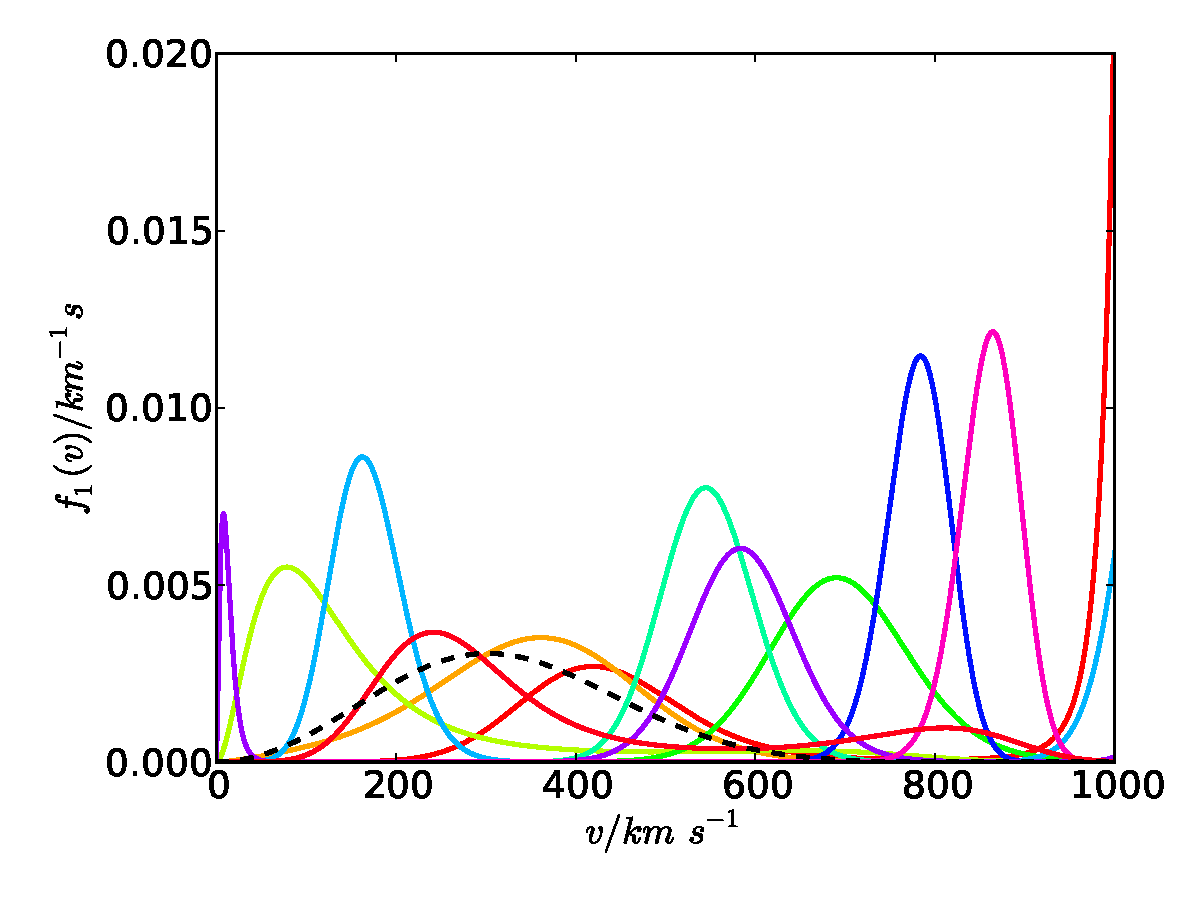
\includegraphics[width=0.75\textwidth]{Poly/Poly.pdf}
  \caption[Examples of $\ln f(v)$ polynomial distributions]{Examples of speed distributions $f_1(v)$ generated using the polynomial parametrisation for $\ln f(v)$ with $N=5$ basis functions. The SHM distribution function in the Earth frame is shown as a black dashed line for comparison.}
  \label{fig:Poly:examples}
\end{figure}

\section{Parameter reconstruction}

\subsection{Experimental benchmarks}
\label{sec:Poly:experiments}
\todo{I can probably shorten this section...Maybe put all the experimental stuff in one place...}
In order to generate mock data sets, we consider three idealized mock experiments, loosely based on detectors which are currently in development. The three target materials we consider here are Xenon, Argon and Germanium. We describe each experiment in terms of its nucleon number $A$, fiducial detector mass $m_\textrm{det}$, efficiency $\epsilon$ and energy sensitivity window $\left[E_\textrm{min}, E_\textrm{max}\right]$. \note{I don't use an `efficiency in Chapter~\ref{ch:Speed}. Why not? Unify them...}

We incorporate the effects of detector sensitivity, analysis cuts and detector down-time into the value of the efficiency $\epsilon$, which we take to be energy independent for simplicity. We consider a total exposure time for all experiments of $t_\textrm{exp} = \textrm{ 2 years}$. The experimental parameter values used in this chapter are summarized in Tab.~\ref{tab:Poly:experiments}. We note that these values may be slightly adjusted or updated compared to those used in Chapter~\ref{ch:Speed} as a result of updated experimental results and projections. We have tried to indicate the source of the values used in Tab.~\ref{tab:Poly:experiments}.

\begin{table}[t]
  \setlength{\extrarowheight}{2pt}
  \begin{center}
%\begin{sideways}
	\begin{tabular}{c|m{1.2cm}m{2.2cm}m{2.1cm}m{2.1cm}}
        \hline\hline
	Experiment  & Target Mass, $A$ & Detector Mass (fid.), $m_\textrm{det}$/kg & Efficiency, $\epsilon$ & Energy Range/keV\\
	\hline
	Xenon  & 131  & 1100 \cite{Aprile:2012a} & 0.7 \cite{Aprile:2012b} & 7-45 \cite{Aprile:2010} \\
	Argon  & 40  & 1000 & 0.9 \cite{Benetti:2007} & 30-100 \cite{Grandi:2005} \\
        Germanium  & 73  & 150 \cite{Bauer:2013b} & 0.6 \cite{Bauer:2013a} & 8-100 \cite{Bauer:2013a} \\
        \hline\hline
	\end{tabular}
%\end{sideways}
  \end{center}
\caption{Summary of experimental parameters used in this work, defined in Sec.~\ref{sec:Poly:experiments}. An exposure of $t_\textrm{exp} = 2 \textrm{ years}$ is used for all 3 experiments.}
\label{tab:Poly:experiments}
\end{table}

The exact parameter values we used in this work do not strongly impact the results we present. However, it is important to note that the total mass and exposure of the experiments will affect the total number of events observed. This in turn will affect the precision of the reconstructions. For example, we have chosen a total Argon mass of 1000 kg. This is the stated target for Argon-based experiments which are in development (e.g. Ref.~\cite{Badertscher:2013}), though at present typical fiducial masses for Argon prototypes are of the order of 100 kg \cite{Grandi:2005}. The data we have generated does not represent the `high-statistics' regime: across all three experiments the total number of events observed is roughly 200-300 with as few as 10 events in the Germanium detector for some scenarios. Using a smaller exposure (or equivalently a smaller interaction cross section) will reduce the precision of the results, but should not introduce any additional bias. We also briefly consider the impact of a \textit{larger} number of events in Sec.~\ref{sec:Poly:Recon}.

\subsection{Theoretical benchmarks}
\label{sec:Poly:benchmarks}

As in Chapter~\ref{ch:Speed}, we assume that SI interactions dominate and use a single value of the interaction cross section $\sigmapsi = 10^{-45} \cmsq$. However, we will consider a range of WIMP masses from 10 GeV, below which the sensitivity of current direct detection experiments decreases dramatically, up to 1000 GeV above which sensitivity to the precise WIMP mass is lost. \todo{Talk at some point about the degeneracy and refer back to it.}

We consider several benchmark speed distributions in this work, including the SHM and the SHM with the addition of a moderate dark disk which accounts for 23\% of the total WIMP density \cite{Pillepich:2014}. For the SHM, we assume a fixed DM density of $\rho_0 = 0.3 \textrm{ GeV cm}^{-3}$. However, we treat the dark disk as an overdensity contributing an \textit{additional} WIMP population, bring the local density up to $\rho_0 = 0.39 \textrm{ GeV cm}^{-3}$ \note{Justify...}. We model the speed distributions as combinations of Gaussian functions in the Earth frame
\begin{equation}
\label{eq:gaussian}
g(\textbf{v}) = N \exp\left(-\frac{(\textbf{v} - \textbf{v}_\textrm{lag})^2}{2\sigma_v^2}\right) \Theta(v_\textrm{esc} - |\textbf{v} - \textbf{v}_\textrm{lag}|)\,,
\end{equation}
where $\textbf{v}_\textrm{lag}$ specifies the peak velocity of the distribution in the Earth frame and $\sigma_v$ the velocity dispersion. We truncate the distribution above the escape speed $v_\textrm{esc} = 544 \kms$. In addition, we also use the speed distribution of Lisanti et al.~\cite{Lisanti:2010}, which has the following form in the Earth's frame:
\begin{equation}
\label{eq:lisanti}
f(\textbf{v}) = N \left[\exp\left(\frac{v_\textrm{esc}^2 - |\textbf{v} - \textbf{v}_0|^2}{k v_0^2}\right) -1\right]^k \Theta(v_\textrm{esc} - |\textbf{v} - \textbf{v}_0|)\,.
\end{equation}
We use the parameter values $k = 2$ and $v_0 = 220 \kms$ in this work. We summarize in Tab.~\ref{tab:Poly:distributions} the different speed distributions considered. We also plot several of these in Fig.~\ref{fig:Poly:Ensemble_distributions} for reference. \note{NB:Time dependence...}

\begin{table}[t]
  \setlength{\extrarowheight}{2pt}
  \setlength{\tabcolsep}{3pt}
  \begin{center}
	\begin{tabular}{m{3cm}|ccc}
        \hline \hline
	Speed distribution benchmark & Fraction & $v_\textrm{lag} / \kms$ & $\sigma_v / \kms$ \\
        \hline
	SHM & 1 & 220 & 156 \\
	\hline
	\multirow{2}{*}{SHM+DD} & 0.77 & 220 & 156 \\
	& 0.23 & 50 & 50 \\
	\hline
	Stream & 1 & 400 & 20 \\
	\hline
	\multirow{2}{*}{Bump} & 0.97 & 220 & 156 \\
	& 0.03 & 500 & 20 \\
	\hline
	\multirow{2}{*}{Double-peak} & 0.5 & 200 & 20 \\
	& 0.5 & 400 & 20 \\
	\hline
	Lisanti et al. & & $v_0 = 220 \kms$ & $k = 2$ \\
        \hline \hline
	\end{tabular}
        
  \end{center}
\caption{Summary of speed distribution benchmarks used in this work. Some benchmarks are modelled as mixtures of two gaussian components (defined in Eq.~\ref{eq:Poly:gaussian}), for which we give the fractional contribution of each component (labelled `Fraction'). The remaining parameters are defined in Eqs.~\ref{eq:Poly:gaussian} and \ref{eq:Poly:lisanti} and the accompanying text. The `bump' and `double-peak' distributions are discussed in Sec.~\ref{sec:Poly:test}.}
\label{tab:Poly:distributions}
\end{table}

\begin{figure}[t]
\centering
  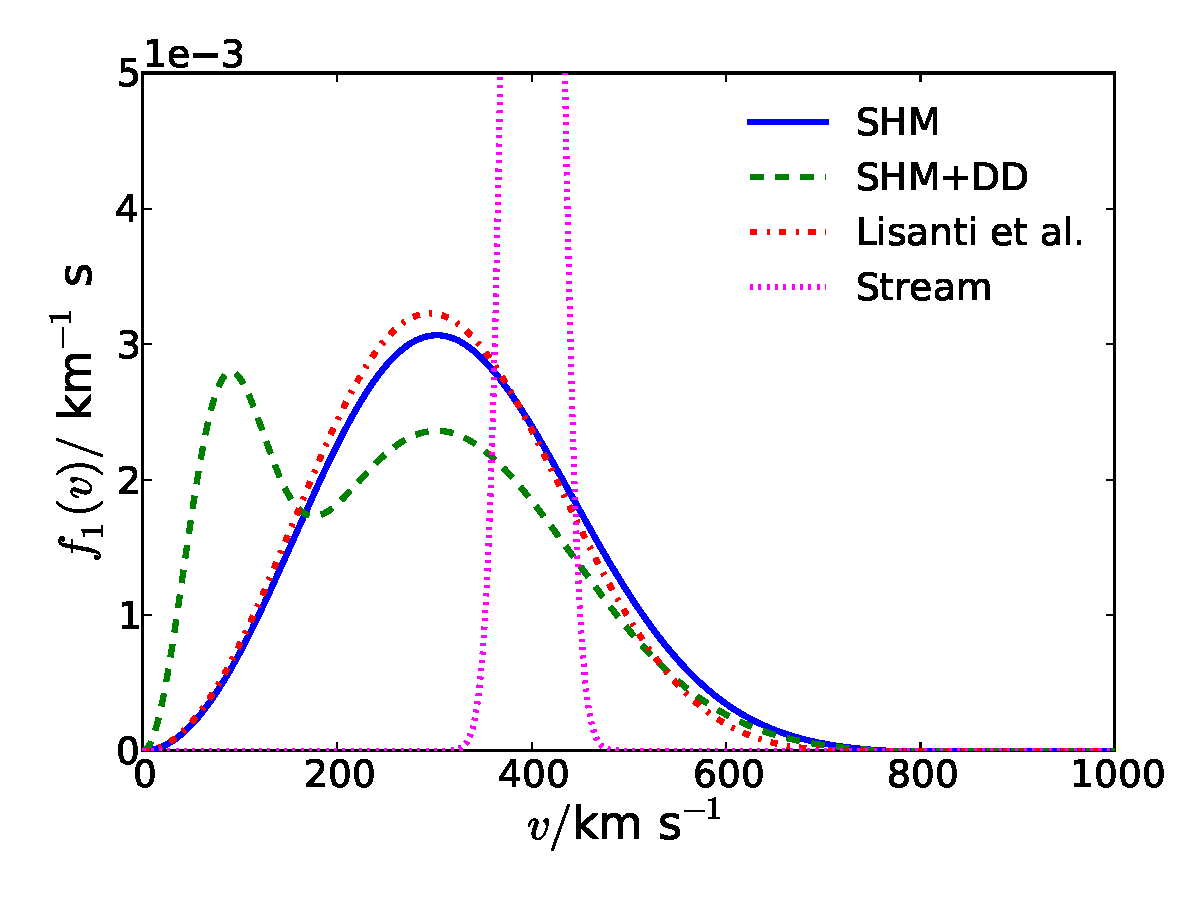
\includegraphics[width=0.75\textwidth]{Poly/SpeedDistributions-Ensemble.pdf}
  \caption{Several of the benchmark speed distributions used in this work. They are defined in Eqs.~\ref{eq:gaussian} and \ref{eq:lisanti} with parameters from Tab.~\ref{tab:Poly:distributions}. These distributions are the SHM (solid blue), SHM+DD (dashed green), Lisanti et al. (dot-dashed red) and the stream (dotted magenta).}
  \label{fig:Poly:Ensemble_distributions}
\end{figure}

\subsection{Parameter sampling}
\label{sec:Poly:ParamRecon}
The parameter space of the speed distribution parameters is now much larger and is poorly explored using conventional MCMC methods. We therefore make parameter inferences using the MultiNest nested sampling package described in Chapter~\ref{ch:ParamRecon}. We summarize the priors used in this work in Tab.~\ref{tab:Poly:priors}. We also summarize in Tab.~\ref{tab:Poly:MultiNest} the MultiNest sampling parameters used.

\begin{table}[t]
  \setlength{\extrarowheight}{2pt}
  \setlength{\tabcolsep}{3pt}
  \begin{center}
	\begin{tabular}{m{1in}|cc}
        \hline\hline
	Parameter & Prior type & Prior range\\
	\hline
	$m_\chi / \textrm{ GeV}$ &  log-flat & $\left[10^{0}, 10^{3}\right]$\\
	$\sigma_p / \textrm{ cm}^2$ & log-flat & $\left[10^{-46}, 10^{-42}\right]$ \\
	$\left\{a_k\right\}$ & linear-flat & $\left[-50, 50\right]$ \\
        $R_{BG} / \textrm{dru}$ & log-flat & $\left[10^{-12}, 10^{-5}\right]$ \\
        \hline\hline
	\end{tabular}
  \end{center}
\caption{Summary of the priors on the parameters used in this work. The background rate $R_{BG}$ is defined in Sec.~\ref{sec:Poly:mass} while the $\left\{a_k\right\}$ are the polynomial coefficients used in the parametrisation.}
\label{tab:Poly:priors}
\end{table}

\begin{table}[t]
  \setlength{\extrarowheight}{2pt}
  \setlength{\tabcolsep}{3pt}
  \begin{center}
	\begin{tabular}{c|c}
        \hline\hline
        Parameter & Value \\
        \hline
	$N_\textrm{live}$ & 10000 \\
	efficiency & 0.25 \\
	tolerance & $10^{-4}$ \\
        \hline\hline
	\end{tabular}
  \end{center}
\caption{Summary of the MultiNest sampling parameters used in this work.}
\label{tab:Poly:MultiNest}
\end{table}

In Sec.~\ref{sec:Poly:stats} and Sec.~\ref{sec:Poly:Recon}, we consider many realisations of data, including the effects of Poisson noise. We therefore use the unbinned likelihood of Eq.~\ref{eq:ParamRecon:unbinnedL} in MultiNest. As in Chapter~\ref{ch:Speed}, make parameter inferences from the marginalised posterior distribution \note{What's the symbol}. We take the mode of the distribution to be the reconstructed parameter value and construct p\% \textit{minimal} credible intervals. This method performs well for small numbers of observations (compared to the number of free parameters in the fit). It is therefore a sensible choice here, where in some cases the number of events observed in an experiment is less than 10. \note{Reorder these paragraphs...?}

In Sec.~\ref{sec:Poly:test} and Sec.~\ref{sec:Poly:mass}, we consider the effects of varying the form of the parametrization and of varying the input WIMP mass. In order to eliminate the effects of Poisson noise, we use Asimov data \cite{Cowan:2013} for these sections. This means that we divide the energy window of each experiment into bins of width 1 keV. We then set the observed number of events $N_{o}^{(i)}$ in bin $i$ equal to the expected number of events $N_{e}^{(i)}$ and use the binned likelihood described by Eq.~\ref{eq:ParamRecon:binnedL}. Here, we have a very large number of observations, namely the exact (non-integer) event numbers in each energy bin. We can therefore use the best fit point as the reconstructed value and construct confidence intervals using the asymptotic properties of the profile likelihood, as described in Sec.~\ref{sec:ParamRecon:freqparams}.
%The profile likelihood can also lead to less noisy reconstructions than the marginalized posterior, especially when the dimensionality of the parameter space becomes high, as in Sec.~\ref{sec:Parametrization} and Sec.~\ref{sec:mass}.
 
\section{Results}

\note{Mention the stream distribution somewhere}

\note{Mention the priors on a - and widening them...}

Before we consider in detail the properties of the parametrisation (including performance as a function of number of basis functions and as a function of input mass), we show some reconstructions using a small numbers of benchmarks. \todo{Show an example - in particular with the \sigmapsi degeneracy - to say that it works - need to show that first. Can't necessarily use the Peter review ones - too many experiments, too few Nlive and not enough basis functions...}


We compare the performance of the polynomial $\ln f(v)$ presented here with the binned distribution functions of the previous chapter. We use a 50 GeV WIMP with a stream distribution function \note{defined where?} and, using a single realisation of data, attempt to reconstruct the WIMP mass using each method. The results are shown in Table~\ref{tab:Poly:ReconstructedMass}. The polynomial $\ln f(v)$ method shows a clear improvement over the other two methods. Not only is the parametrised distribution smooth, removing the need for any fixed lengthscales, but it is also better able to capture the rapidly varying form of the stream distribution function. \note{Redo this, I don't think I want to use the stream...}

\begin{table}[t]
  \setlength{\extrarowheight}{5pt}
  \begin{center}
	\begin{tabular}{lc}
         \hline\hline
	 Parametrisation & Reconstructed mass (GeV) \\
	 \hline
	 Polynomial $\ln f(v)$ & \(44.7^{+6.9}_{-3.6}\) \\
	 Binned $f(v)$ & \(29.3^{+0.4}_{-1.0}\) \\
	 Binned $\tilde{f}(p)$ & \(38.2^{+1.6}_{-2.3}\)\\
         \hline\hline
	\end{tabular}
  \end{center}
  \caption{Reconstructed mass using the parametrization presented in this chapter, as well as the the speed binning and momentum binning methods of Chapter~\ref{ch:Speed} for comparison. The benchmark used is a stream distribution function described in \note{Somwhere!} and a 50 GeV WIMP. In all cases, 5 speed distribution parameters (either bins or basis coefficients) are used.}
\label{tab:Poly:ReconstructedMass}
\end{table}

We will now explore in more detail the properties of this new parametrisation method.

\subsection{Testing the parametrisation}
\label{sec:Poly:test}

We now consider the two questions: \begin{inparaenum} \item how many basis functions are required and \item which polynomial basis should be used? \end{inparaenum} In order to answer these questions, we use the two benchmark distribution functions illustrated in Fig.~\ref{fig:Poly:VaryingN_distributions}. We have chosen these benchmarks not because they are necessarily realistic distribution functions but because they should be difficult to fit using standard techniques and fitting functions (e.g.~\cite{Lisanti:2010}). The first distribution (referred to as `bump') is a SHM distribution with the addition of a small bump, which contributes just 3\% of the total WIMP population and could correspond to a small sub-halo or stream \cite{Vogelsberger:2009}. This should be difficult to fit because it represents only a very small deviation from the standard scenario. The second distribution (referred to as `double-peak') has a sharp and rapidly varying structure, which we anticipate should be difficult to capture using a small number of basis functions.

\begin{figure}[t]
\centering
  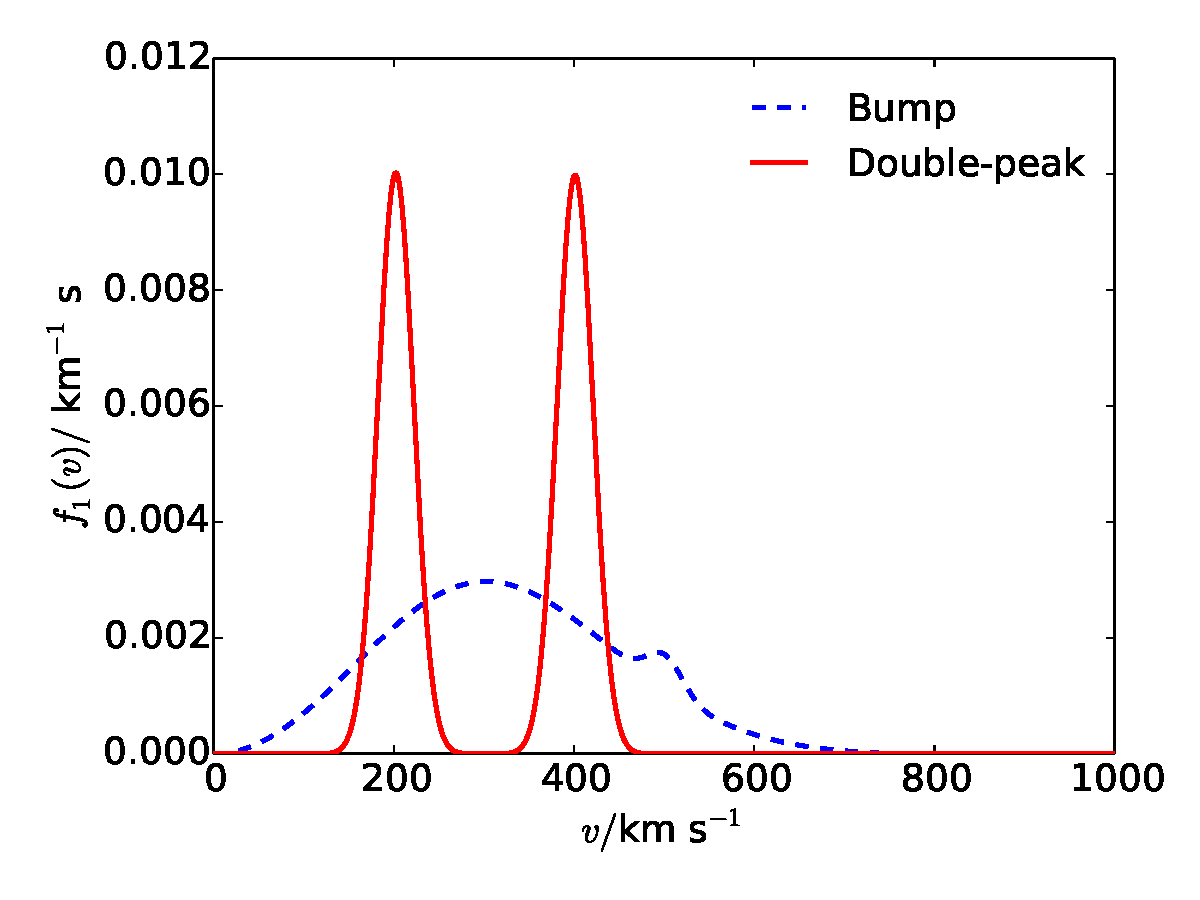
\includegraphics[width=0.75\textwidth]{Poly/SpeedDistributions-VaryingN.pdf}
  \caption{Benchmark speed distributions used in Sec.~\ref{sec:Poly:test} to test the performance of the parametrization as a function of the number and type of basis functions.}
  \label{fig:Poly:VaryingN_distributions}
\end{figure}

\subsubsection{Varying the number of basis functions}

We first investigate how the reconstructed WIMP mass $m_\textrm{rec}$ and uncertainty varies with the number of basis functions $N$. For now, we fix our choice of basis to shifted Legendre polynomials:
\begin{equation}
P_k(v) = L_k\left(2\frac{v}{v_\textrm{max}} - 1\right)\,,
\end{equation}
where $L_k$ is the Legendre polynomial of order $k$, and $v_\textrm{max}$ is a cut off for the parametrization.
 
The lower panel of Fig.~\ref{fig:Poly:BUMP_LEG} shows the best fit mass and 68\% confidence intervals as a function of $N$, using as input a WIMP of mass 50 GeV and the `bump' distribution function. The reconstructed mass very rapidly settles close to the true value, using as few as three basis functions. This is because adding the bump near $v \sim 500 \kms$ still leaves the mean inverse speed relatively smooth, so a large number of basis function are not required. The correct mass is reconstructed and we emphasize in the lower panel of Fig.~\ref{fig:Poly:BUMP_LEG} that the reconstruction is stable with the addition of more basis functions.

We should also consider how the quality of the fit changes as a function of $N$. We would expect that adding fit parameters should always lead to a better fit. Eventually, the fit should be good enough that adding additional basis functions will no longer improve it significantly. We can then be confident that our reconstruction is accurate and not an artifact of using too few basis functions. In order to investigate this, we utilise the Bayesian Information Criterion (BIC) \cite{Schwarz:1978}, which is given by:

\begin{equation}
BIC = 2N_p\textrm{ln}(N_m) - \textrm{ln}(\mathcal{L}_\textrm{max}) \, ,
\end{equation}
where $N_p$ is the number of free parameters, $N_m$ is the number of measurements or observations and $\mathcal{L}_\textrm{max}$ is the maximum likelihood value obtained in the reconstruction. For the case of binned data, $N_m$ corresponds simply to the total number of energy bins across all experiments. This criterion penalises the inclusion of additional free parameters and in comparing several models, we should prefer the one which minimises the BIC.

\begin{figure}[t]
\centering
  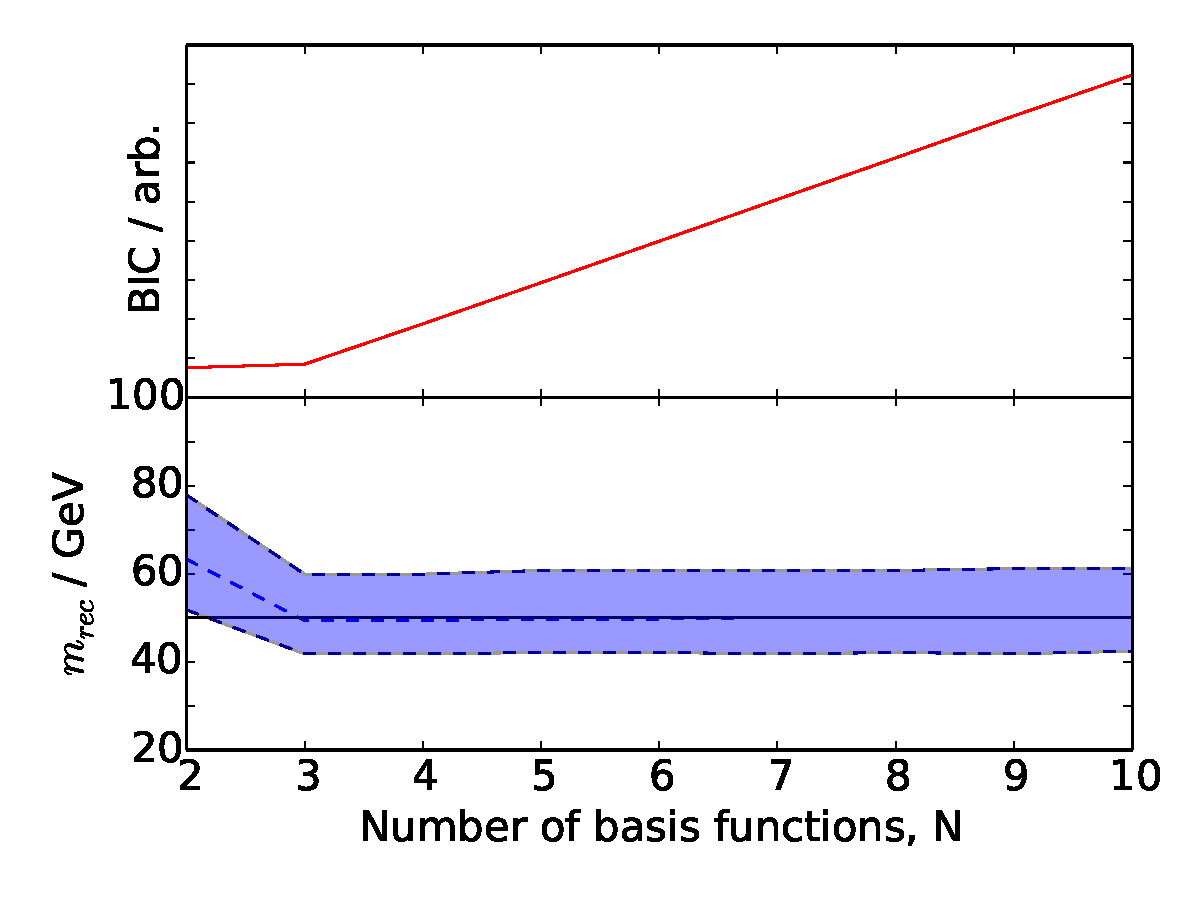
\includegraphics[width=0.75\textwidth]{Poly/VaryingN_BUMP_LEG.pdf}
  \caption{Bayesian information criterion (BIC) as a function of the number of basis functions for an underlying `bump' distribution function, 50 GeV WIMP and using Legendre polynomial basis functions (upper panel). Also shown (lower panel) are the reconstructed WIMP mass (dashed blue line), 68\% confidence interval (shaded blue region) and underlying WIMP mass (solid horizontal black line).}
  \label{fig:Poly:BUMP_LEG}
\end{figure}

The upper panel of Fig.~\ref{fig:Poly:BUMP_LEG} shows the BIC (in arbitrary units) as a function of the number of basis functions for the `bump' distribution function. The BIC is comparable for the cases of $N=2$ and $N=3$, indicating that the quality of the fit is improved slightly by the addition of another basis function. However, adding further basis functions does not have a significant impact on the maximum likelihood, leading to an increase in the BIC. This coincides with the stabilization of the reconstructed mass around the true value and we conclude that only two or three basis functions are required to provide a good fit to the data.

Figure \ref{fig:Poly:DP_LEG} shows the corresponding results for the `double-peak' distribution function. Here, we note that the bias induced by using too small a number of basis functions is larger than for the case of the `bump' distribution, due to the more complicated structure in this case. The BIC is minimized for $N=7$, indicating that additional basis functions do not significantly improve the quality of the fit to data. This suggests that the shape of the speed distribution can be well fit by $N\geq7$ basis functions. As shown in the lower panel of Fig.~\ref{fig:Poly:DP_LEG}, the reconstruction of the WIMP mass is stable around the true mass for these values of $N$.

\begin{figure}[t]
\centering
  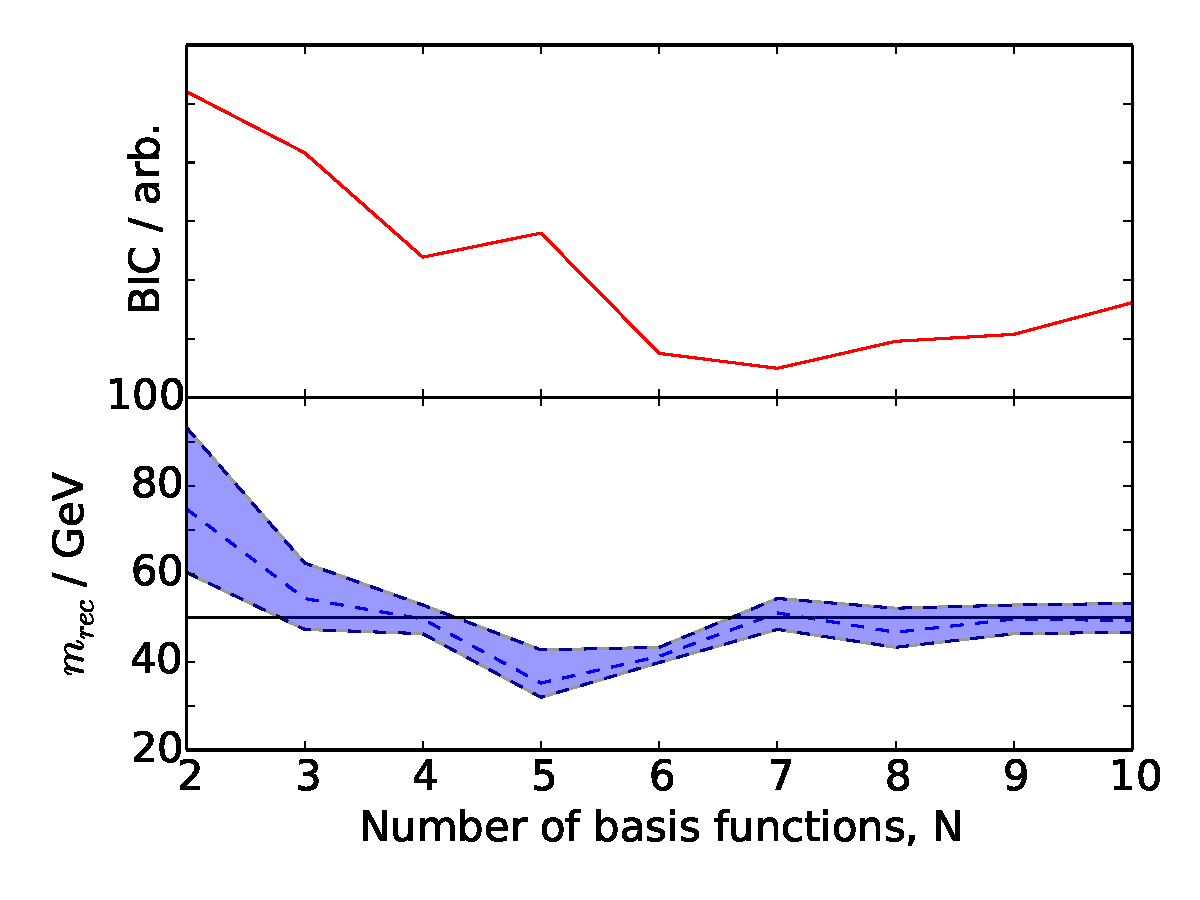
\includegraphics[width=0.75\textwidth]{Poly/VaryingN_DP_LEG.pdf}
  \caption{As Fig.~\ref{fig:Poly:BUMP_LEG} but for an underlying `double-peak' distribution function.}
  \label{fig:Poly:DP_LEG}
\end{figure}

We propose that such a procedure should be used in the case of real data should a dark matter signal be observed at multiple detectors. We have shown that by analyzing the reconstructed mass as a function of $N$ we can recover the true mass and that by using the BIC we can be confident that we have obtained an adequate fit to data.

\subsection{Choice of basis functions}

We now consider the second question posed at the start of Sec.~\ref{sec:Poly:parametrisation}: which polynomial basis should be used? As previously mentioned, we test two different polynomial bases: Legendre and Chebyshev polynomials. \note{Beef this section up and copy some of the `chebyshev is used often for approximation' stuff down here...}

We have checked that the reconstruction results using Chebyshev polynomials are largely indistinguishable from the case of Legendre polynomials for both the `bump' and `double-peak' distributions and as a function of $N$. This leads us to conclude that the accuracy of the reconstruction is independent of the specific choice of basis. However, the reconstruction was much faster in the case of the Chebyshev basis. This is illustrated in Fig.~\ref{fig:Poly:times}, which shows the time taken for reconstruction of the `bump' benchmark as a function of $N$. The time taken grows much more slowly for the Chebyshev basis (roughly as $N^2$) than for the Legendre basis (roughly as $N^3$). We have also checked that this difference is not an artifact of how we calculate the basis functions. These results indicate that this choice of basis provides both reliable and efficient reconstruction for the WIMP mass and we therefore use the Chebyshev basis in the remainder of this work.

\begin{figure}[t]
\centering
  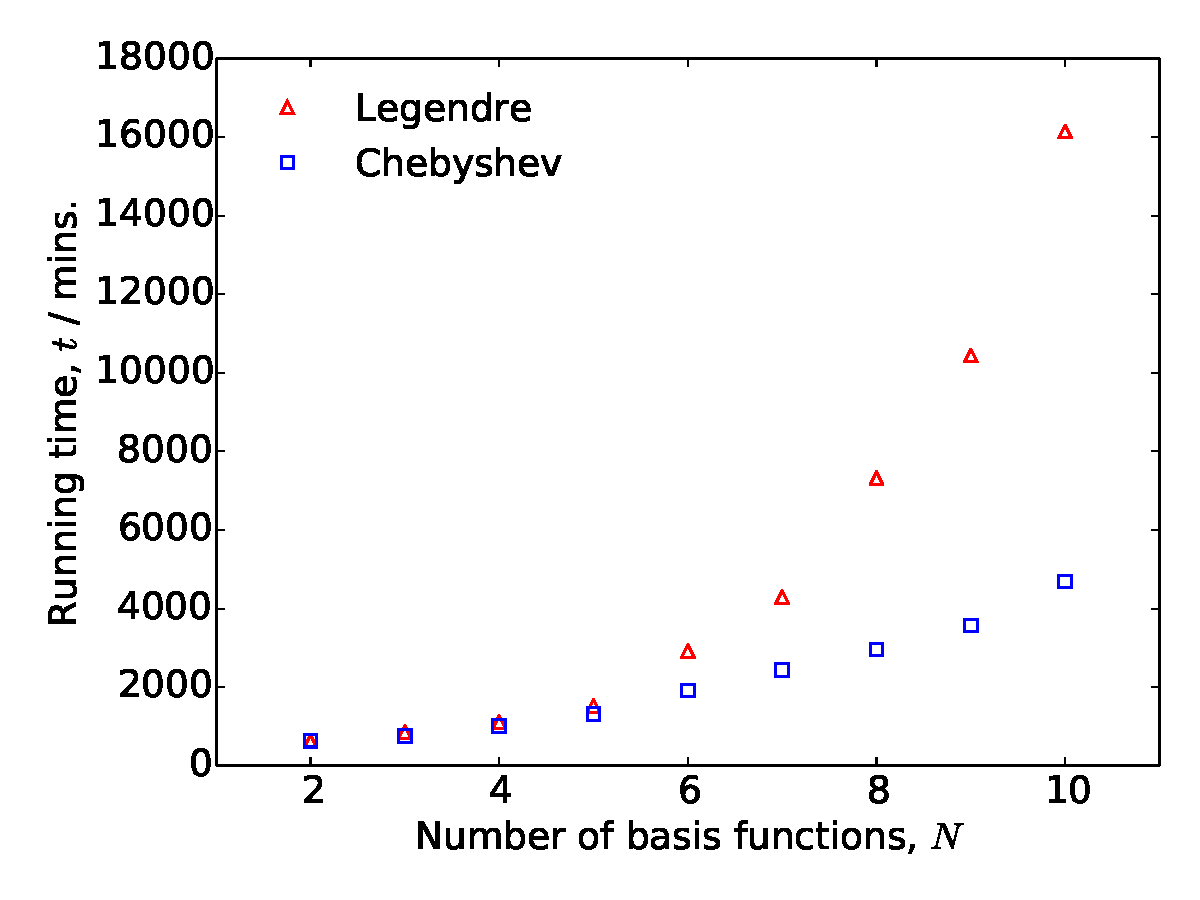
\includegraphics[width=0.75\textwidth]{Poly/RunTimes.pdf}
  \caption{Time taken (using 4 processors in parallel) for the reconstruction of the `bump' benchmark, as a function of number of basis functions. The time taken using the Chebyshev basis (blue squares) grows more slowly with $N$ than for the Legendre basis (red triangles).}
  \label{fig:Poly:times}
\end{figure}

\section{Varying $m_\chi$}
\label{sec:Poly:mass}

We now consider the performance of the parametrisation over a wide range of WIMP masses. We generate Asimov data for WIMP masses of 10, 20, 30, 40, 50, 75, 100, 200 and 500 GeV and reconstruct the best fit WIMP mass $m_\textrm{rec}$ and 68\% and 95\% confidence intervals from the profile likelihood. We use the SHM as a benchmark distribution function and use a fixed number of $N=5$ basis functions. The results are shown in Fig.~\ref{fig:Poly:VaryingM}, along with the line $m_\textrm{rec} = m_\chi$ for reference.

For large values of $m_\chi$, the shape of the event spectrum becomes independent of $m_\chi$ \cite{Green:2008}, which results in a widening of the confidence intervals as the WIMP mass increases. For low mass WIMPs, fewer events are observed in each bin, again resulting in wider confidence intervals. It should be noted that for this analysis we have used Asimov data, in which the exact (non-integer) number of events is recorded in each bin. For low mass WIMPs, this means that the spectrum (and therefore the correct WIMP mass) is still well reconstructed using Asimov data, in spite of the small number of events. The tightest constraints are obtained when the input WIMP mass is close to the masses of several of the detector nuclei (in the range 30-80 GeV). There also appears to be no bias in the WIMP mass: the reconstruction matches the true mass across all values considered.

\begin{figure}[t]
\centering
  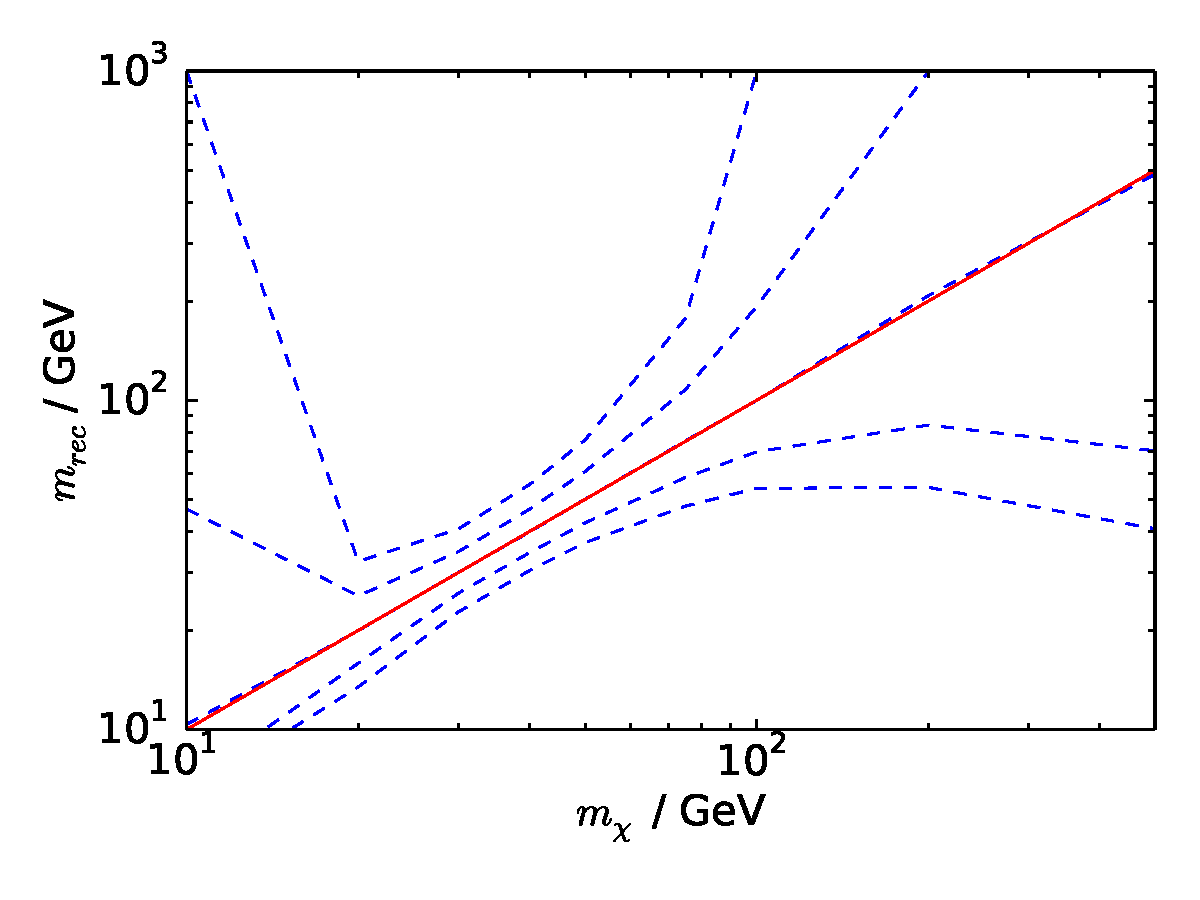
\includegraphics[width=0.75\textwidth]{Poly/VaryingM.pdf}
  \caption{Reconstructed WIMP mass $m_\textrm{rec}$ (central dashed blue line) as a function of input WIMP mass $m_\chi$ as well as 68\% and 95\% intervals (inner and outer blue dashed lines respectively). The line $m_\textrm{rec} = m_\chi$ (solid red line) is also plotted for reference.}
  \label{fig:Poly:VaryingM}
\end{figure}

As described in Chapter~\ref{ch:Speed}, for low mass WIMPs the momentum distribution may be very narrow, owing to their lower momenta. However, if we wish to parametrise the full momentum range to which the experiments are sensitive, this would be much wider. \note{Better explanation...?} The momentum parametrization method therefore performs poorly for low mass WIMPs. The parametrization presented in this chapter does not suffer from similar problems.

So far, we have only considered idealized direct detection experiments. We now apply the method to more realistic mock detectors, taking into account the effects of finite energy resolution, as well as unrejected background events. We assume here that each experiment has a gaussian energy resolution with fixed width $\sigma_E = 1 \textrm{ keV}$, such that the observed event rate for recoils of energy $E$ is given by: \note{Do I say this in a previous chapter?}

\begin{equation}
\frac{\textrm{d}R}{\textrm{d}E} = \int_{0}^{\infty} \frac{1}{\sqrt{2 \pi} \sigma_E}\exp\left\{-\frac{(E-E')^2}{2\sigma_E^2}\right\} \frac{\textrm{d}{R'}}{\textrm{d}E'} \, \textrm{d}E'\,,
\end{equation}
where the primed event rate is the underlying (perfect resolution) rate. We also assume a constant flat background rate for each experiment $R_\textrm{BG} = 10^{-6}$ events/kg/keV/day (which has been suggested as a possible background rate for Xenon1T \cite{Aprile:2010} and WArP-100L \cite{Grandi:2005}) when generating mock data sets. However, we allow the flat background rate in each experiment to vary as free parameters during the fit.

We have chosen relatively generic resolution and background parameters in this work, because the precise details of energy resolution and background shape and rate will depend on the specific experiment under consideration. Instead, we hope to show that the inclusion of more realistic experimental setups does not introduce an additional bias or otherwise spoil the good properties of the method presented here.

Figure \ref{fig:Poly:VaryingM_real} shows the reconstructed mass as a function of input mass in this more realistic scenario. The 68\% and 95\% confidence intervals are now wider and the reconstructed mass does not appear to be as accurate. For input masses above $\sim$100 GeV, the uncertainties become very wide, with only a lower limit of $m_\textrm{rec} > 20 \textrm{ GeV}$ being placed on the WIMP mass.  Due to the poorer energy resolution the shape of the energy spectrum is less well-determined. In addition, a flat background contribution can mimic a higher mass WIMP, as it leads to a flatter spectrum. This leads to a strong degeneracy, as a wide range of mass values can provide a good fit to the data. For high input masses, the profile likelihood is approximately constant above $m_\textrm{rec} \sim 20 \textrm{ GeV}$, indicating that there is no sensitivity to the underlying WIMP mass.

In spite of this, the true mass values still lie within the 68\% and 95\% confidence intervals. In addition, the poor values for the reconstructed mass for heavy WIMPs are a side effect of the loss of sensitivity. Because the profile likelihood is approximately flat, the maximum likelihood point is equally likely to be anywhere within the 68\% interval. These effects would be present even if we had considered a fixed form for the speed distribution. However, when we allow for a range of possible speed distributions, the effects become more pronounced. These results show that for more realistic experimental scenarios, the method presented in this paper remains reliable over a range of masses, though its precision may be significantly reduced.

\begin{figure}[t]
\centering
  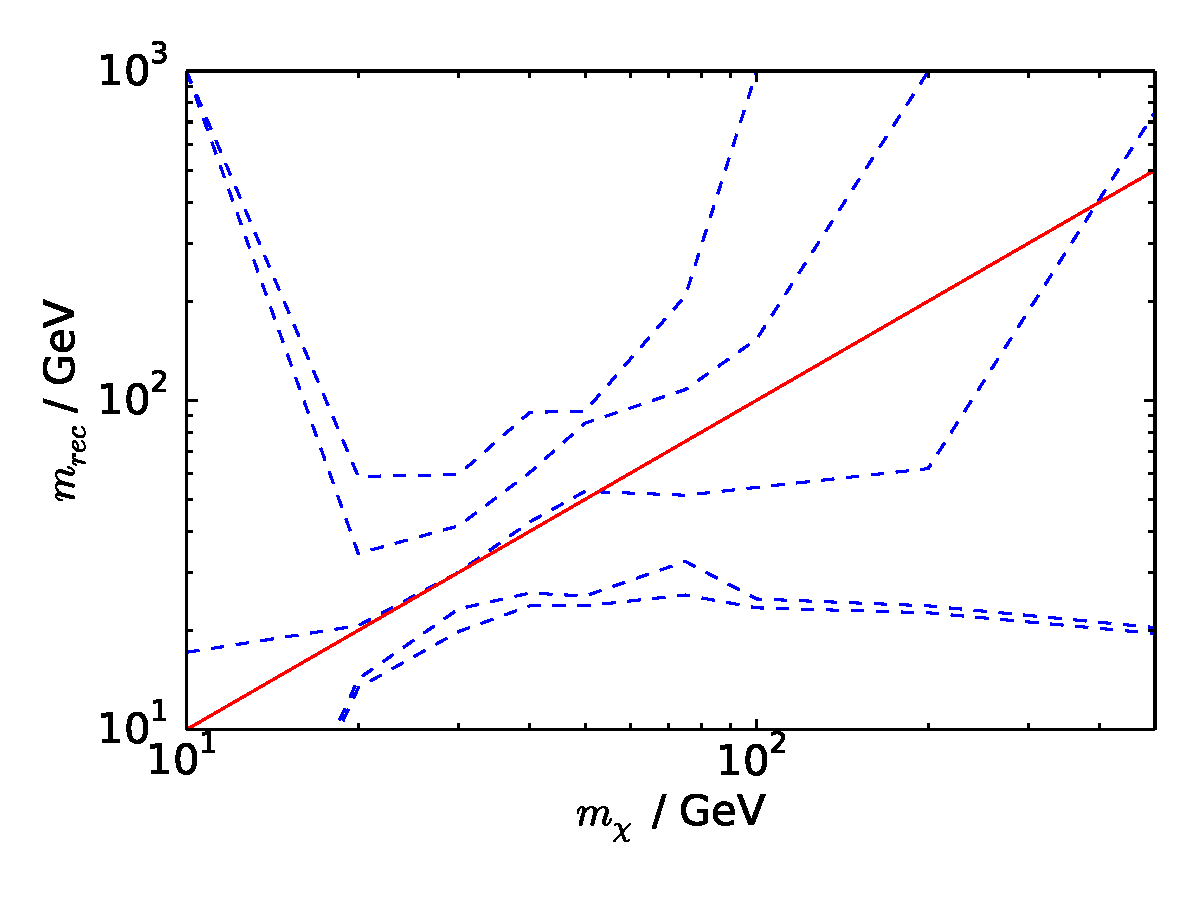
\includegraphics[width=0.75\textwidth]{Poly/VaryingM_real.pdf}
  \caption{As fig.~\ref{fig:Poly:VaryingM} but including the effects of finite energy resolution and non-zero backgrounds, as described in the text.}
  \label{fig:Poly:VaryingM_real}
\end{figure}

\section{Statistical properties}
\label{sec:Poly:stats}

\todo{Include the coverage maps...}

We now consider the impact of statistical fluctuations on the reconstruction of the WIMP mass. In reality, the number of events observed $N_o$ at a given experiment will be Poisson distributed about the expected value $N_e$, while the observed distribution of recoil energies will not exactly match that expected from the calculated event rate. The fundamental statistical limitations of future direct detection experiments have been studied in detail in Ref.~\cite{Strege:2012}. As in Chapter~\ref{ch:Speed}, we generate 250 realisations of data from the mock experiments described in Tab.~\ref{tab:Poly:experiments}. Each realisation of the mock data is generated as follows: \note{Move this to the previous chapter...}

\begin{enumerate}
\item Calculate the number of expected events $N_e$, given $\left\{m_\chi, \sigma_p, f(v)\right\}$, using Eq.~\ref{eq:N_expected},
\item Pick the number of observed events $N_o$ from a Poisson distribution with mean $N_e$,
\item Pick recoil energies $\left\{E_1, E_2, ..., E_{N_o}\right\}$, from the distribution $P(E)$ in Eq.~\ref{eq:eventdistribution},
\item Repeat for all three experiments.
\end{enumerate}

For each realisation, we then use the method described in Sec.~\ref{sec:Poly:ParameterRecon} (using $N = 5$ basis functions) to reconstruct the WIMP mass and 68\% and 95\% credible intervals. Figure~\ref{fig:Poly:Realisations} shows the distribution of reconstructed masses for an input mass of 50 GeV for three benchmark speed distributions: SHM, SHM+DD and Lisanti et al.\, as described in Sec.~\ref{sec:Poly:benchmarks}. In all three cases, the reconstructions are peaked close to the true value, regardless of the underlying distribution. For the SHM+DD distribution, the spread of reconstructions is slightly wider (with more reconstructions extending up to higher masses). This is due to the smaller number of events for this benchmark, making the data sets more susceptible to Poisson fluctuations.

In order to assess the accuracy of the reconstructed value of the mass $m_\textrm{rec}$, we also calculate the bias $b$ for each realisation:

\begin{equation}
\label{eq:Poly:bias}
b = \textrm{ln}(m_\textrm{rec} / \textrm{GeV}) - \textrm{ln}(m_\textrm{true} / \textrm{GeV})\,.
\end{equation}
We compare the logarithms of the mass values because we have used logarithmically-flat priors on the WIMP mass. In Tab.~\ref{tab:Poly:bias} we show the average bias across all 250 realisations for each of the three benchmark distributions. In all three cases, the average bias is consistent with zero. Even in the SHM+DD case, which shows larger fluctuations away from the true value, there is no statistical bias.

\begin{figure}
\centering
  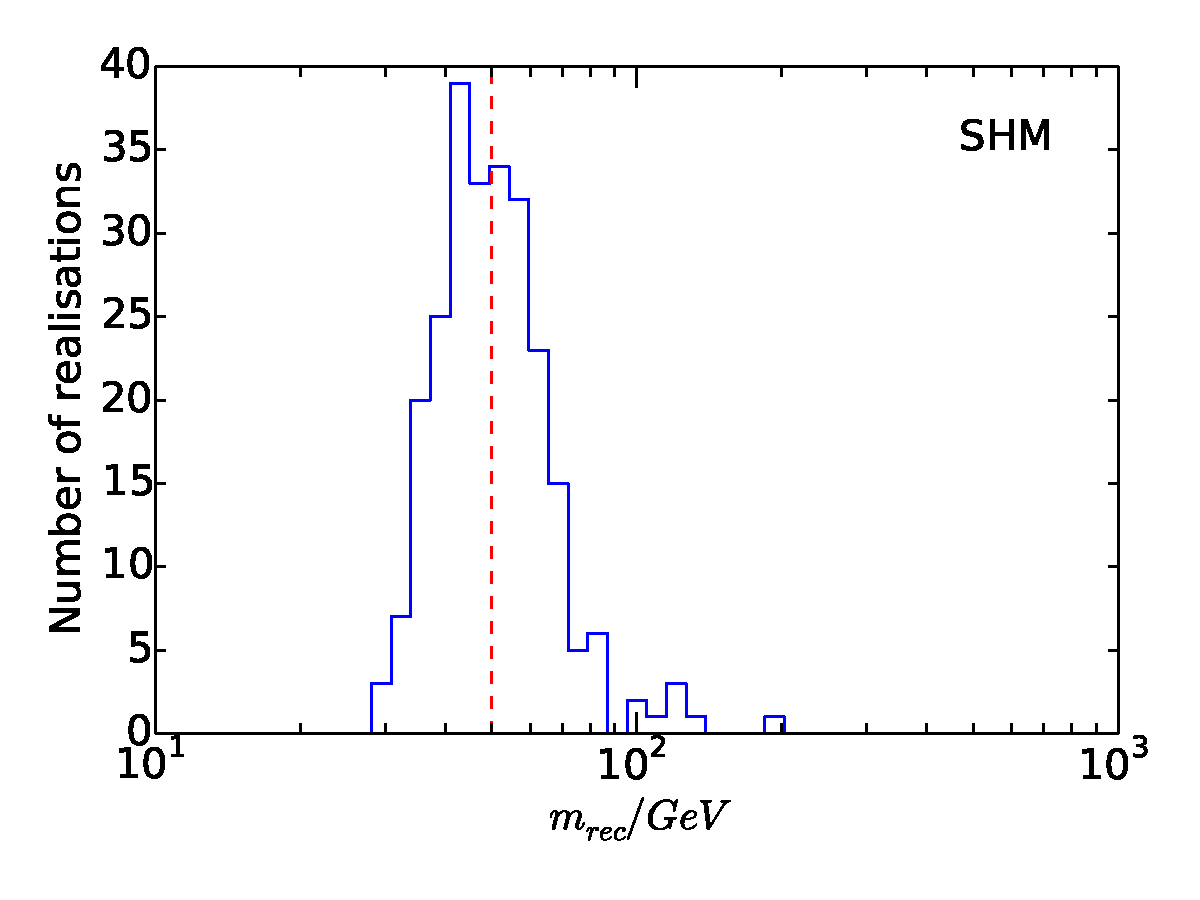
\includegraphics[trim=0cm 1cm 0cm 0.5cm,clip=true,width=0.75\textwidth]{Poly/SHM_ensemble.pdf}
  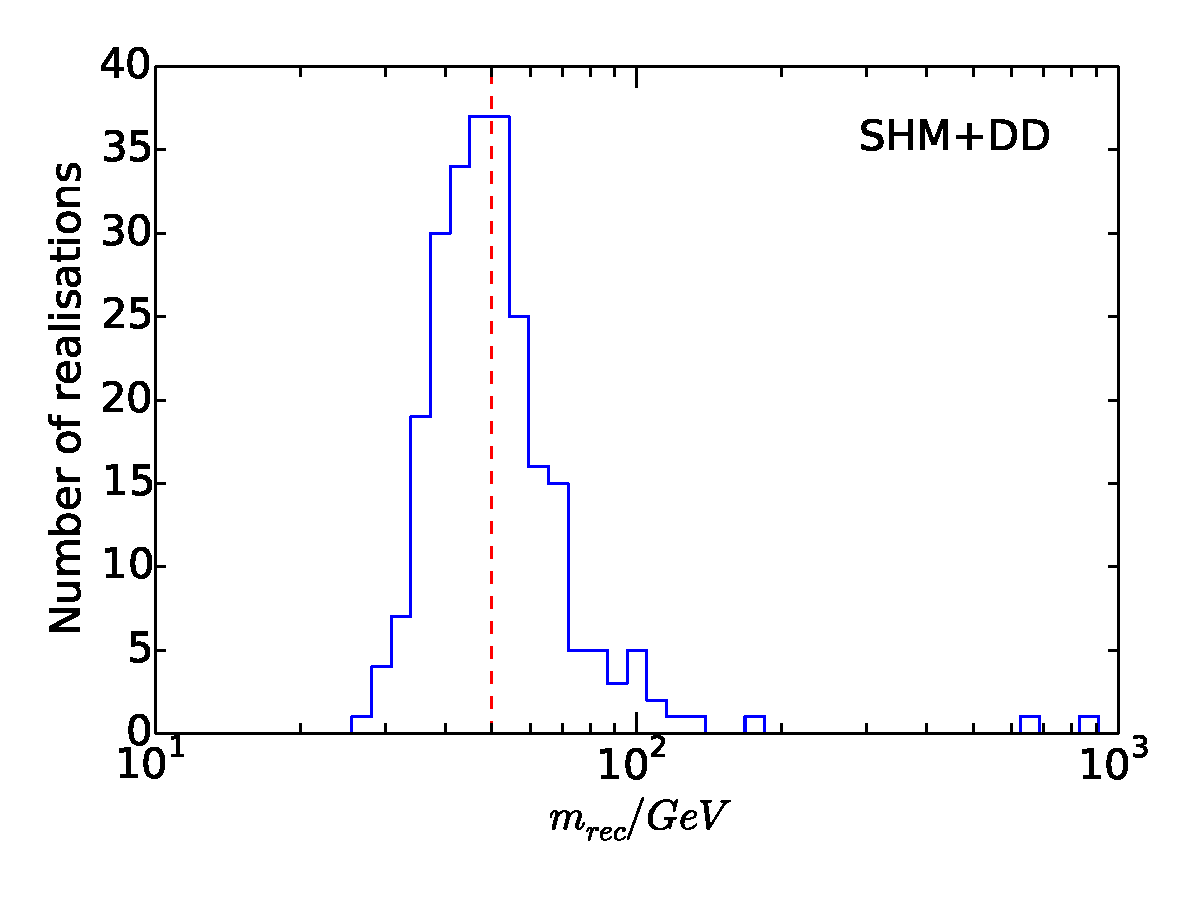
\includegraphics[trim=0cm 1cm 0cm 0.5cm,clip=true,width=0.75\textwidth]{Poly/DD_ensemble.pdf}
  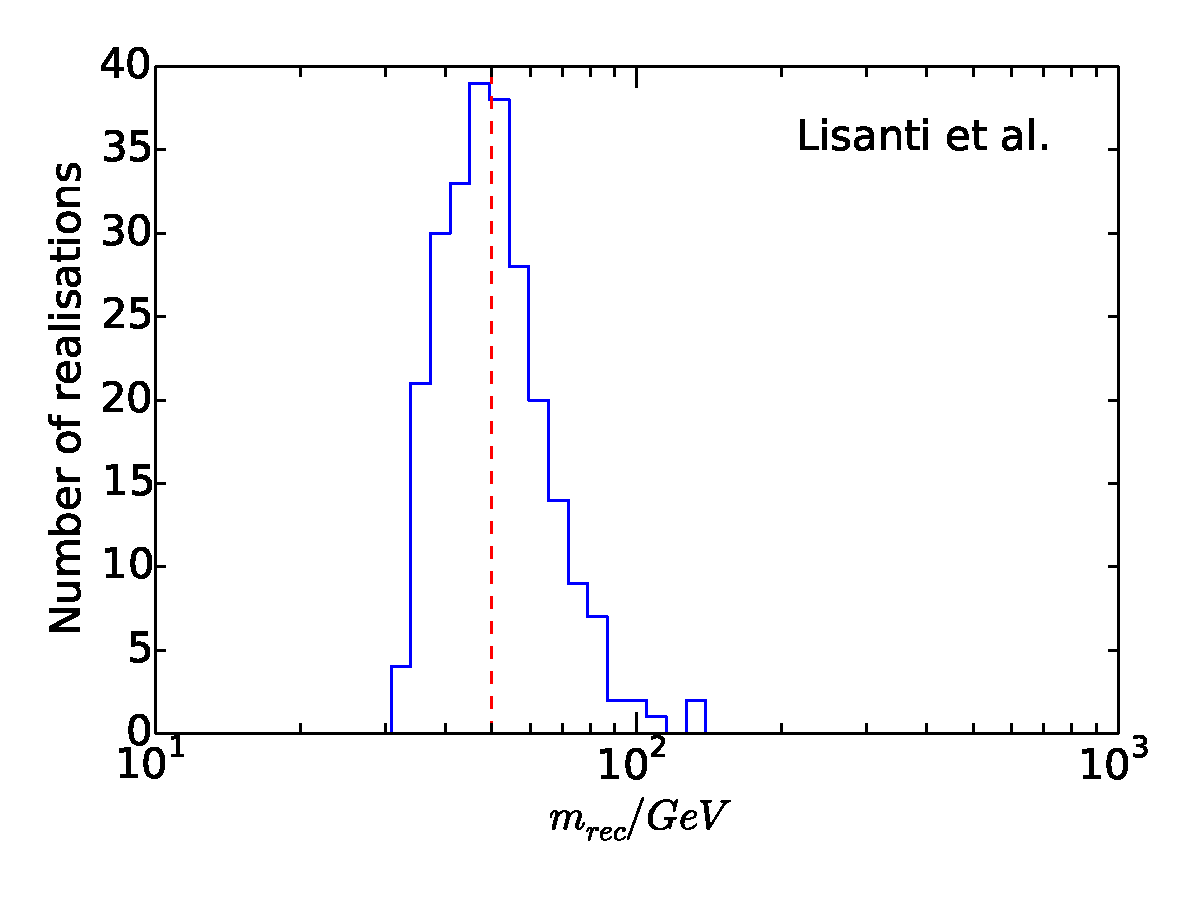
\includegraphics[trim=0cm 1cm 0cm 0.5cm,clip=true,width=0.75\textwidth]{Poly/LIS_ensemble.pdf}
  \caption{Distribution of the reconstructed mass $m_\textrm{rec}$ for 250 mock data sets generated using several benchmark speed distributions, defined in Sec.~\ref{sec:Poly:benchmarks}. These are the SHM (top), SHM+DD (middle) and Lisanti et al.\ (bottom) distributions. The input WIMP mass of $m_\chi = 50 \textrm{ GeV}$ is shown as a vertical dashed red line.}
  \label{fig:Poly:Realisations}
\end{figure}

\begin{table}[t]
  \setlength{\extrarowheight}{3pt}
  \setlength{\tabcolsep}{3pt}
  \begin{center}
	\begin{tabular}{c|c}
        \hline\hline
	Benchmark speed distribution & Mean bias $\langle b \rangle$ \\
	\hline
	SHM & 0.002 $\pm$ 0.008 \\
	SHM+DD & 0.005 $\pm$ 0.007 \\
	Lisanti et al. & 0.01 $\pm$ 0.01 \\
        \hline\hline
	\end{tabular}
  \end{center}
\caption{Mean bias $\langle b \rangle$ in the reconstructed log WIMP mass (Eq.~\ref{eq:Poly:bias}). This was calculated over 250 realisations using three different benchmark speed distributions.}
\label{tab:Poly:bias}
\end{table}

We also test the \textit{coverage} of the credible intervals which have been constructed. \note{Refer back to the section on coverage.} Table \ref{tab:Poly:coverage} shows the coverage values for the $68\%$ and $95\%$ intervals obtained in this section. In each case, there is very close to exact coverage. We have also checked that these intervals only provide exact coverage for the true WIMP mass of 50 GeV. Other values of $m_\textrm{rec}$ are contained within the intervals less frequently than the true value, again indicating that this parametrization allows for unbiased and statistically robust reconstructions of the WIMP mass.

\begin{table}[t]
  \setlength{\extrarowheight}{3pt}
  \setlength{\tabcolsep}{3pt}
  \begin{center}
	\begin{tabular}{m{1in}|cc}
        \hline\hline
	Benchmark speed distribution & 68\% coverage & 95\% coverage\\
	\hline
	SHM &  71 $\pm$ 3 \% & 94 $\pm$ 3 \%  \\
	SHM+DD & 68 $\pm$ 3 \% & 91 $\pm$ 4 \%  \\
	Lisanti et al. & 70 $\pm$ 3 \% & 95 $\pm$ 3 \%  \\
        \hline \hline
	\end{tabular}
  \end{center}
\caption{Coverage of 68\% and 95\% credible intervals calculated from 250 data realisations each for three benchmark speed distributions. The concept of coverage is described in the text of Sec.~\ref{sec:Poly:stats}.}
\label{tab:Poly:coverage}
\end{table}

\section{Reconstructing $f_1(v)$}
\label{sec:Poly:Recon}

Using the method described in this paper, we can obtain the posterior probability distribution for the coefficients $\left\{ a_1, ..., a_{N-1}\right\}$ given the data, which we refer to as $P(\textbf{a})$. We would like to be able to present this information in terms of the distribution function $f_1(v)$ in order to compare with some known distribution or look for particular features in the distribution. However, due to the fact that the distribution function is normalized, the values of $f_1$ at different speeds will be strongly correlated. We illustrate here how robust comparisons with benchmark distributions can be made.

As a first step, we can attempt to sample from the $P(\textbf{a})$, in order to obtain $P(f_1(v))$. This is the probability distribution for the value of $f_1$ at a particular speed $v$, marginalizing over the values of $f_1$ at all other speeds. We can repeat for a range of speeds to obtain 68\% and 95\% credible intervals for the whole of $f_1(v)$. The result of this procedure is presented in Fig.~\ref{fig:Poly:f}, for a randomly selected realisation from the SHM ensemble of Sec.~\ref{sec:Poly:stats}. The underlying SHM distribution is shown as a solid line, while the 68\% and 95\% marginalized intervals are shown as dark and light shaded regions respectively. In this naive approach, we see that there is little shape information which can be recovered from the reconstruction, with only upper limits being placed on the speed distribution.

\begin{figure}[t]
\centering
  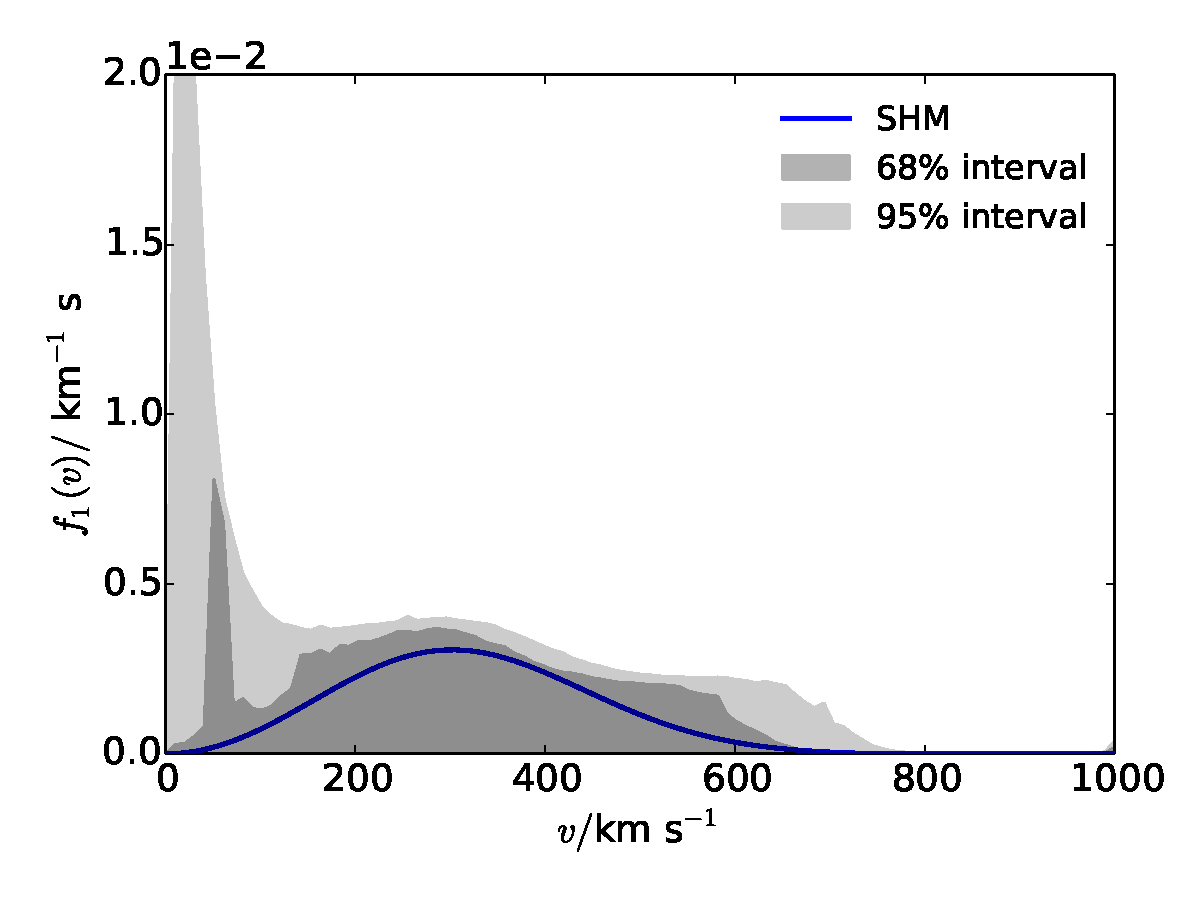
\includegraphics[width=0.75\textwidth]{Poly/f_SHM.pdf}
  \caption{Reconstructed speed distribution for a single realisation of data, generated for a 50 GeV WIMP. 68\% and 95\% credible intervals are shown as dark and light shaded regions respectively, while the underlying SHM distribution function is shown as a solid blue line.}
  \label{fig:Poly:f}
\end{figure}


This method performs poorly because, as initially mentioned in Sec.~\ref{sec:Poly:ParamRecon}, we have no information about the fraction of dark matter particles below the energy threshold of our experiments. If this fraction is large, the event rate for a given cross-section is suppressed. However, increasing the cross-section will increase the total event rate. There is thus a degeneracy between the shape of the speed distribution and the cross-section, meaning that we can only probe the shape of $f_1(v)$, rather than its overall normalization. This degeneracy has not been accounted for in Fig.~\ref{fig:Poly:f}. We can attempt to correct for this by adjusting the normalization of $f_1(v)$. If we fix $f_1(v)$ to be normalized to unity above $v_a$ (where $v_a \approx 171 \kms$ is the lowest speed probed by the experiments for a WIMP of mass 50 GeV), we can compare the shapes of the underlying and reconstructed distribution functions. This is illustrated in Fig.~\ref{fig:Poly:f_scaled}, which shows that we now broadly reconstruct the correct shape of $f_1(v)$. Below $v_a$, the value of $f_1(v)$ is poorly constrained, because the experiments provide no information about the shape of the distribution below theshold.

There remain several issues with this approach. In order to utilize this method, we must know the approximate value of the lowest speed probed by the experiments. However, this value is set by the WIMP mass. We could determine $v_a$ using the reconstructed WIMP mass, but this would be subject to significant uncertainty. In addition, direct reconstructions of the speed distribution are easily biased. The upper limit of the energy windows of the experiments corresponds to a particular WIMP speed (for a given WIMP mass). WIMPs above this speed still contribute to the total event rate, but contribute no spectral information. The reconstructed shape of the high speed tail of the distribution is therefore not constrained by the data, but may affect the reconstructed value of $f_1$ at lower speeds.


\begin{figure}[t]
\centering
  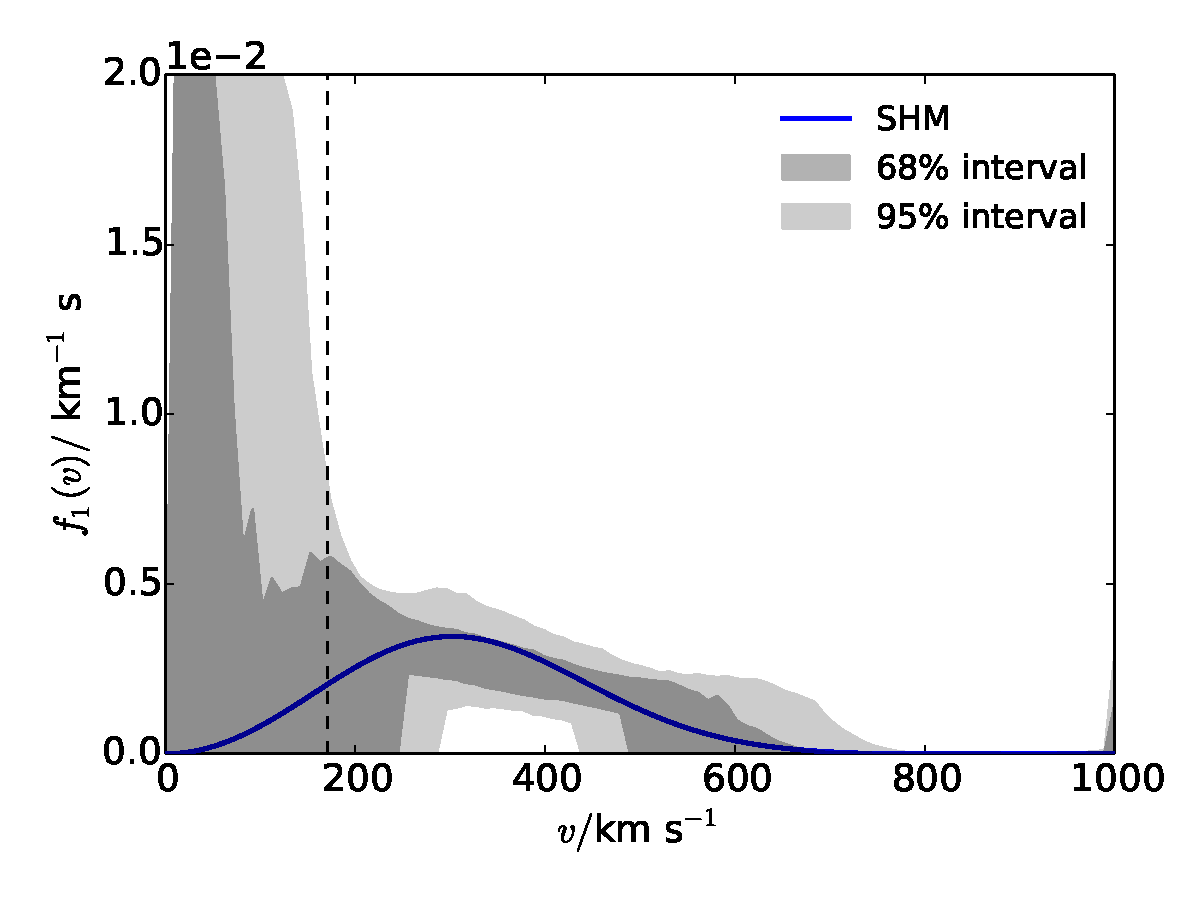
\includegraphics[width=0.75\textwidth]{Poly/f_SHM_scaled_line.pdf}
  \caption{Reconstructed speed distribution for the same realisation of data as Fig.~\ref{fig:Poly:f}. In this case, we have also normalized $f_1(v)$ to unity above $v_a \approx 171 \kms$ (vertical dashed line). This is the lowest speed accessible to the experiments for a WIMP of mass 50 GeV. 68\% and 95\% credible intervals are shown as dark and light shaded regions respectively, while the underlying SHM distribution function is shown as a solid blue line.}
  \label{fig:Poly:f_scaled}
\end{figure}

An alternative approach is to reconstruct the mean inverse speed $\eta(v)$ (defined in Eq.~\ref{eq:eta}) at some speed $v$. Because $\eta(v)$ is an integral function of $f_1$, it is less prone to bias as it takes into account the full shape of the distribution at speeds greater than $v$. However, we do not know the normalization of $f_1$ and so we must normalize $\eta$ appropriately. For each point sampled from $P(\textbf{a})$, we calculate $\eta$. We then divide by $\alpha(v)$, the fraction of WIMPs above speed $v$, calculated using the same parameter point:
\begin{equation}
\label{eq:alpha}
\alpha(v) = \int_{v}^{\infty} f_1(v') \, \textrm{d}v'\,.
\end{equation}

We will write this rescaled mean inverse speed as $\eta^*(v) = \eta(v)/\alpha(v)$. The value of $\eta^*(v)$ is a measure of the shape of the distribution function above $v$. However, information about the normalization of the distribution has been factored out by dividing by $\alpha(v)$. We no longer need to know the value of $v_a$ in order to obtain information about the shape of the distribution at higher speeds. We may still need to decide the speed down to which we trust our reconstruction, but this no longer relies on an arbitrary choice of $v_a$ to normalize the reconstructions at all speeds.

In Fig.~\ref{fig:Poly:eta_stats}, we plot the mean reconstructed value of $\eta^*$ at several values of $v$, using 250 realisations of the 50 GeV SHM benchmark. We also show the mean upper and lower limits of the 68\% credible intervals as errorbars. The form of $\eta^*$ for the SHM is shown as a solid blue line. In all cases except for $v=100 \kms$, the mean reconstructed value is close to the true value, indicating that $\eta^*$ can be reconstructed without bias using this method. At low speeds, the reconstructed value deviates from the true value. In addition, the credible intervals lead to \textit{under}coverage in the $v=100 \kms$ case. However, this point lies below the lowest speed to which the experiments are sensitive and therefore we cannot trust the reconstruction at this low speed. We have checked that for the remaining values of $v$ the method provides exact or overcoverage, indicating that at higher speeds we can use $\eta^*$ as a reliable and statistically robust measure of the shape of the distribution.

\begin{figure}[t]
\centering
  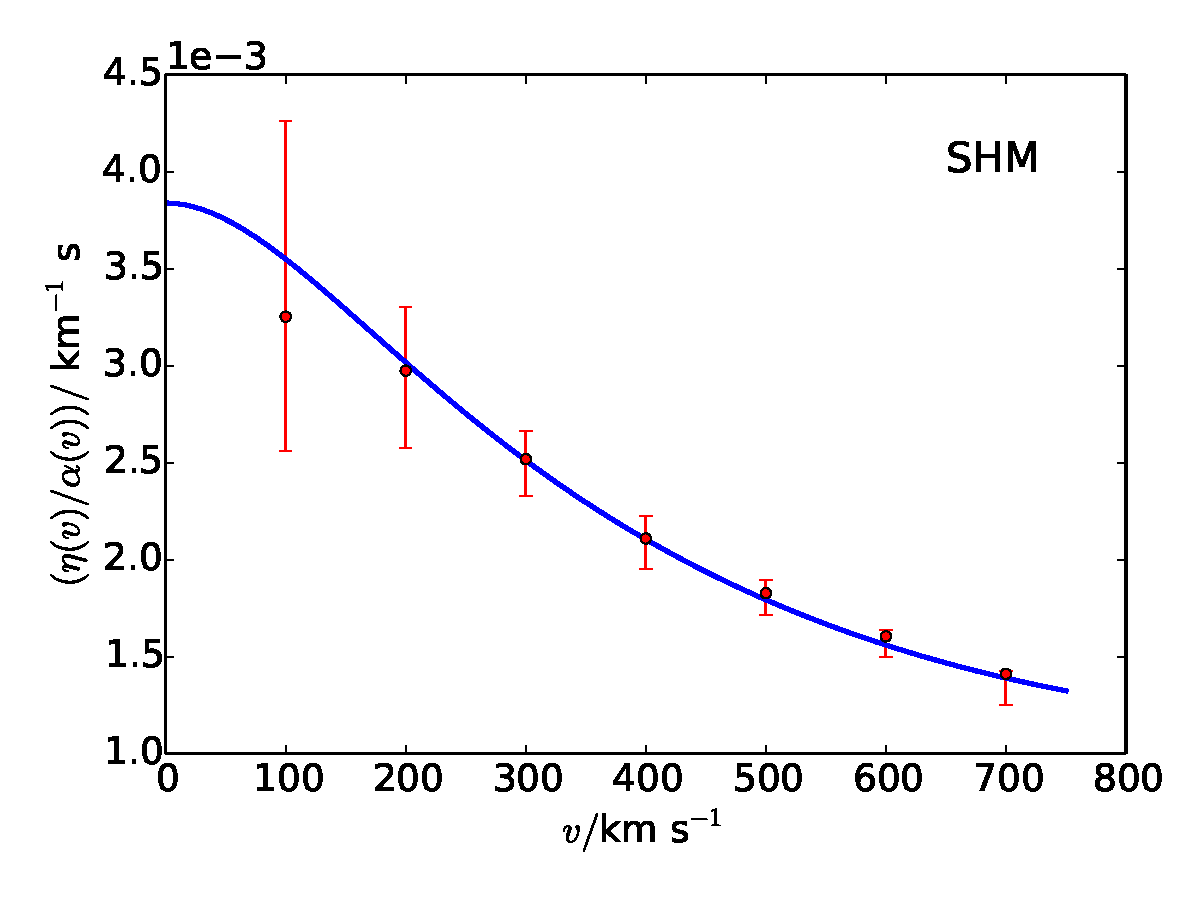
\includegraphics[width=0.75\textwidth]{Poly/Eta.pdf}
  \caption{Mean reconstructed values of the rescaled mean inverse speed $\eta(v)/\alpha(v)$ at several values of $v$, calculated over 250 realisations of data using a 50 GeV WIMP and underlying SHM distribution function. Errorbars indicate the mean upper and lower limits of the 68\% credible intervals. The underlying form of $\eta(v)/\alpha(v)$ obtained from the SHM is shown as a solid blue line.}
  \label{fig:Poly:eta_stats}
\end{figure}


In the case of a single realisation of data, we would like to compare the probability distribution for $\eta^*(v)$ (obtained from $P(\textbf{a})$) to the value calculated from some test distribution. We note that several distributions may produce the same value of $\eta^*(v)$ at a given value of $v$. Thus, we may fail to reject a distribution function which is not the true distribution. However, if the calculated value of $\eta^*(v)$ does lie outside the $p\%$ interval, we can reject it at the $p\%$ level.

\note{Make sure I don't confuse the definitions of $\alpha$...}

We can increase the discriminating power of this method by repeating this reconstruction over all speeds and checking to see if the benchmark value of $\eta^*$ is rejected at any value of $v$. The result of this procedure is shown in Fig.~\ref{fig:Poly:eta} for a single realisation of data generated using an SHM distribution (the same data as in Figs. \ref{fig:Poly:f} and \ref{fig:Poly:f_scaled}). We plot the 68\%, 95\% and 99\% credible intervals as shaded regions, as well as the values of $\eta^*(v)$ calculated from several benchmark speed distribution. We will focus on the intermediate speed range ($v \gtrsim 200 \kms$), as we do not know \textit{a priori} the lowest speed to which the experiments are sensitive.


\begin{figure}[t]
\centering
  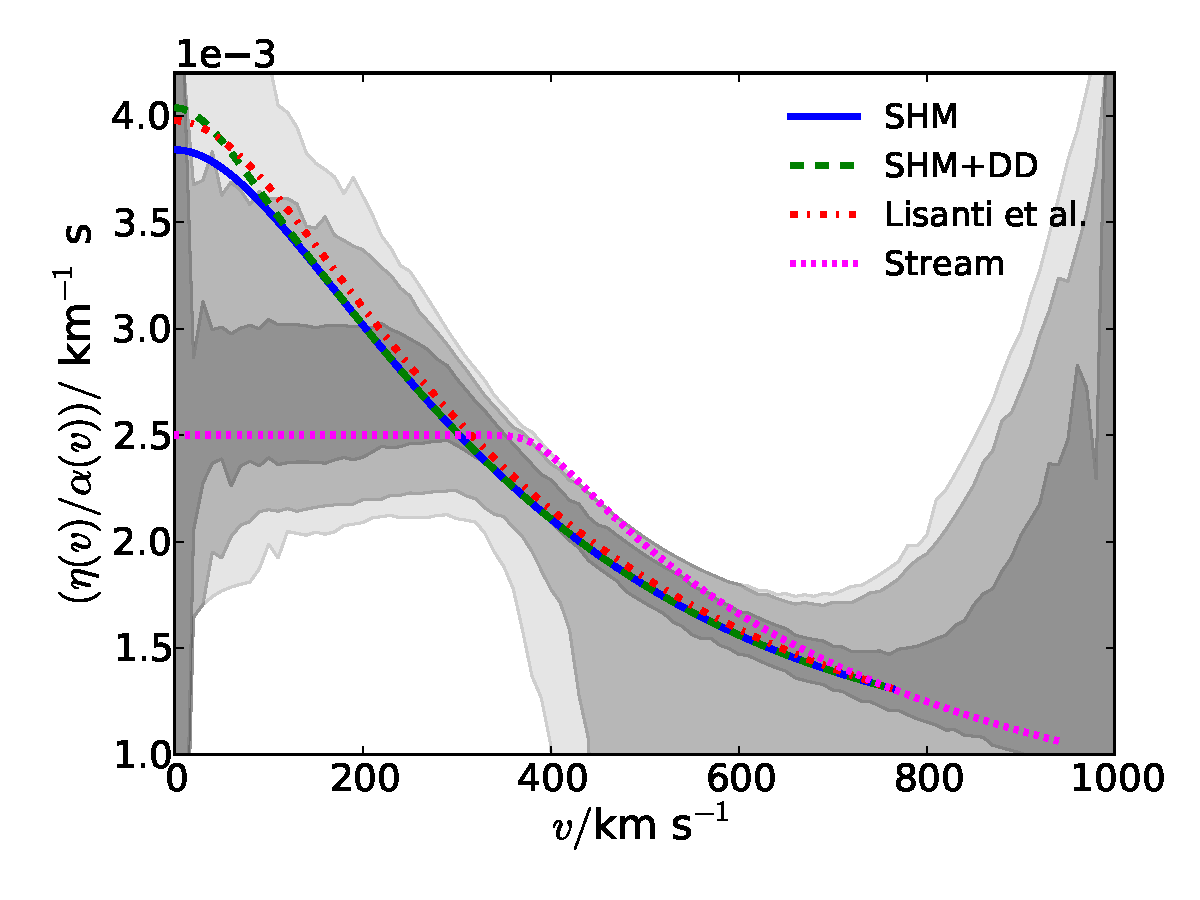
\includegraphics[width=0.75\textwidth]{Poly/SHM_lores.pdf}
  \caption{Rescaled mean inverse speed $\eta(v)/\alpha(v)$, reconstructed from a single realisation of data using a 50 GeV WIMP and underlying SHM distribution function. At each value of $v$ we calculate 68\%, 95\% and 99\% credible intervals (shown as shaded intervals). We also show the calculated values of $\eta(v)/\alpha(v)$ for several possible benchmark speed distributions: SHM (solid blue), SHM+DD (dashed green), Lisanti et al.\ (dot-dashed red) and stream (dotted magenta). The benchmark curves are truncated when the underlying distribution function goes to zero.}
  \label{fig:Poly:eta}
\end{figure}

The reconstructed intervals are consistent with a range of possible distribution functions. The SHM and SHM+DD distributions are identical over a wide range of speeds. This is because above $\sim 200 \kms$, the two distributions differ in normalization but not in shape. Differences appear between the two at low speeds where their shapes diverge. The Lisanti et al.\ distribution results in a larger deviation from the SHM, but not sufficiently large to differentiate between the two distributions given the size of the uncertainties. Finally, the stream distribution results in a significantly different form for $\eta^*(v)$. At approximately $400 \kms$, the curve for the stream distribution lies outside the reconstructed 99\% credible interval. We can therefore use this method to reject the stream distribution at the 99\% confidence level.

Figure \ref{fig:Poly:eta_hires} shows the results of a reconstruction using a larger exposure. In this case, we generate data using the Lisanti et al.\ distribution and an exposure increased by a factor of $2.5$, resulting in approximately 1000 events across the three detectors. As expected, the resulting credible intervals are now substantially narrower. The stream distribution now lies significantly outside the 99\% interval. In Fig.~\ref{fig:Poly:eta_hires_zoom}, we show the same results, but focusing in on the region around $v \sim 400 \kms$. At certain points, the SHM and SHM+DD distributions now lie outside the 95\% credible interval, suggesting that with a number of events of the order of 1000, we may be able to reject these benchmarks.

\begin{figure}[t]
\centering
  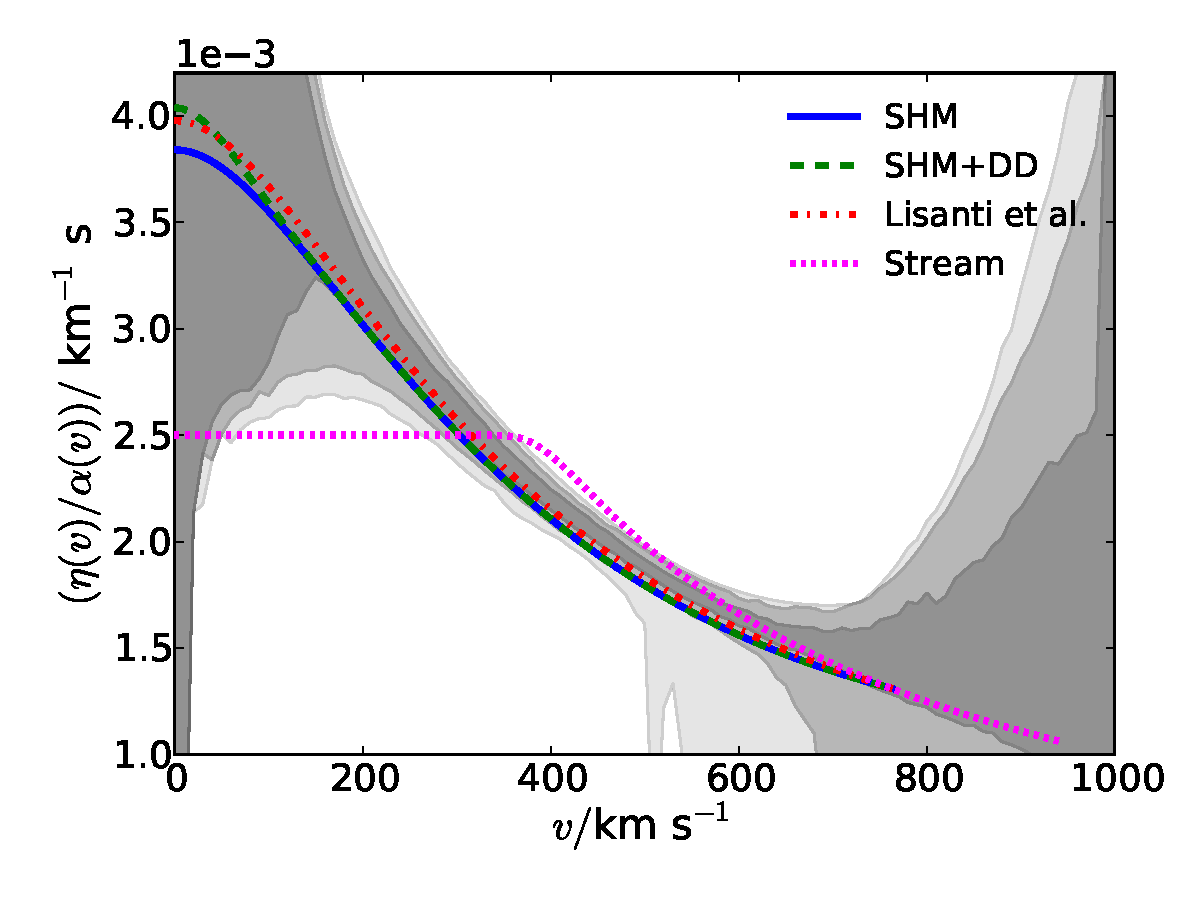
\includegraphics[width=0.75\textwidth]{Poly/LIS_hires.pdf}
  \caption{As Fig.~\ref{fig:Poly:eta}, but using as input a Lisanti et al.\ speed distribution and an exposure time which is 2.5 times longer.}
  \label{fig:Poly:eta_hires}
\end{figure}


\begin{figure}[t]
\centering
  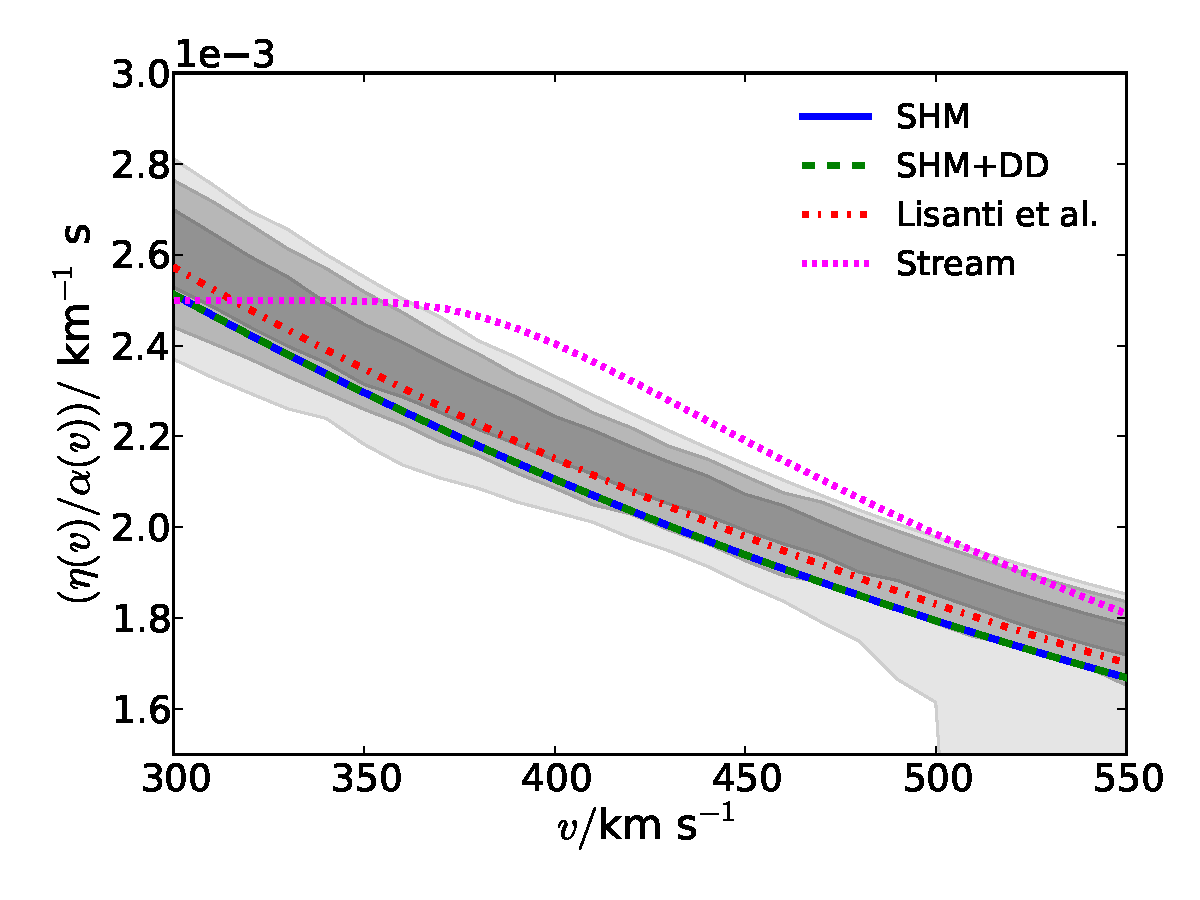
\includegraphics[width=0.75\textwidth]{Poly/LIS_hires_zoom.pdf}
  \caption{As Fig.~\ref{fig:Poly:eta_hires}, but focusing on the region around $v \sim 400 \kms$. Notice that in the range $400-550 \kms$, both the SHM and SHM+DD curves lie at or below the lower limit of the 95\% credible interval.}
  \label{fig:Poly:eta_hires_zoom}
\end{figure}

While the method displayed in Fig.~\ref{fig:Poly:f_scaled} allows the approximate shape of the speed distribution to be reconstructed, reconstructions of $\eta^*(v)$ allow more statistically robust statements to be made about the underlying speed distribution. In particular, Fig.~\ref{fig:Poly:eta_hires_zoom} illustrates that with larger exposures deviations from Maxwellian speed distributions can be detected in a model-independent fashion.

\label{sec:Conclusions}

We have studied in detail a new parametrization for the local dark matter speed distribution, which provides a significant improvement over previous model-independent parametrisations. This method involves writing the logarithm of the speed distribution as a polynomial in speed $v$ and fitting the polynomial coefficients (along with the WIMP mass and cross section) to the data. We have attempted to disentangle in this paper the influence of  different benchmark speed distributions, different benchmark WIMP masses and different forms for the parametrization. \note{These conclusions may be a little wordy...} We summarize our conclusions as follows:

\begin{itemize}

\item We have shown that the reconstruction of the WIMP mass is robust under changes in the number of basis functions $N$. We have used the Bayesian Information Criterion (BIC) to compare models with different values of $N$ and have shown that minimizing the BIC allows us to determine how many basis functions are required for a reliable reconstruction. We have also demonstrated that the results of the method do not depend strongly on the choice of basis functions, but that the speed of reconstructions may improved by using the Chebyshev polynomial basis.

\item We have shown that the method leads to unbiased reconstructions of the WIMP mass for masses in the range 10-500 GeV. Including realistic experimental parameters, including non-zero backgrounds and finite energy resolution, reduces the precision of these reconstructions. In particular, for large values of the input mass, we can only place a lower limit of approximately 20 GeV on the reconstructed mass. This is significantly lower than in the idealized case, where we can typically constrain the WIMP mass to be heavier than around 50 GeV.

\item We have used several ensembles of data realisations to demonstrate the statistical properties of the method, including unbiased reconstructions and exact coverage of the WIMP mass.

\item We have presented several ways of displaying the reconstructed WIMP speed distribution using this method. In order to make robust statistical inferences about the speed distribution, we calculate the probability distribution of $\eta(v)/\alpha(v)$. This is the mean inverse speed $\eta(v)$, which appears in the direct detection event rate (eq.~\ref{eq:Rate}), rescaled by the fraction of WIMPs $\alpha(v)$ above speed $v$. This can be used as a measure of the \textit{shape} of the distribution function, from which the unknown normalization has been factored out. We can then compare to the expected value of $\eta(v)/\alpha(v)$ from a given benchmark speed distribution, allowing us to distinguish between different underlying models.
\end{itemize}

It should be noted that due to the finite threshold energies of direct detection experiments, we cannot probe the low speed population of WIMPs. If we make no assumptions, we have no information about the form of $f(v)$ below threshold and therefore little information about the overall normalisation of $f(v)$. This translates to an unavoidable degeneracy in the WIMP interaction cross section \sigmapsi. 

In spite of this, we have shown that the method allows for a robust determination of the WIMP mass over a large range of input parameters, both in terms of particle physics and astrophysics. The inclusion of more realistic experimental parameters does not introduce any additional bias, but does reduce the precision of reconstructions. Finally, we have shown that we can distinguish different forms of the speed distribution. With around 1000 events, it may be possible to detect minor deviations from the Standard Halo Model and begin to search for more interesting structure in the speed distribution of the Milky Way.

